%!TEX TS-program = xelatex

\documentclass[aspectratio=169]{beamer}

\newbool{russian}
\booltrue{russian}
\usepackage{HSE-theme/beamerthemeHSE}

\usepackage[english,russian]{babel}
\usepackage{amsmath}
\usepackage[no-math]{fontspec}
\IfFontExistsTF{HSE Sans}{
    \setsansfont{HSE Sans}
}{
    \setsansfont{CMU Sans Serif}
}
\IfFontExistsTF{Courier New}{
    \setmonofont{Courier New}
}{
    \setmonofont{Latin Modern Mono}
}

\uselanguage{russian}
\languagepath{russian}
\deftranslation[to=russian]{Theorem}{Теорема}
\deftranslation[to=russian]{Definition}{Определение}
\deftranslation[to=russian]{Definitions}{Определения}
\deftranslation[to=russian]{Corollary}{Следствие}
\deftranslation[to=russian]{Fact}{Факт}
\deftranslation[to=russian]{Example}{Пример}
\deftranslation[to=russian]{Examples}{Примеры}

\usepackage{graphicx}
\usepackage{booktabs}
\usepackage{array}
\usepackage{colortbl}
\usepackage{tikz}
\usetikzlibrary{calc}
\graphicspath{{assets/}{images/}{../Копия «Новый проект» (7)/graphics/}{../Копия «Новый проект» (7)/graphics/figures/}}
\newcommand{\litrefs}[1]{\vfill{\scriptsize\textit{Источники:} #1}}
\newcommand{\crossouttext}[1]{%
\tikz[baseline=(X.base)]{
\node[inner sep=0pt,outer sep=0pt] (X) {#1};
\draw (X.south west) -- (X.north east);
\draw (X.north west) -- (X.south east);
}%
}
\newcommand{\MetricLegend}{%
\vfill
{\fontsize{6.8}{8}\selectfont
	\begin{itemize}
		\setlength{\itemsep}{0.01cm}
		\item \textit{BinaryAcc} --- точность бинарного различения исходных и искажённых графов.
		\item \textit{IntraAcc} --- точность упорядоченных пар \textit{clean/corrupted} в рамках одного трека.
		\item \textit{InterAcc} --- точность упорядоченных пар \textit{clean/corrupted} с разными треками.
	\end{itemize}
}
}

\title[Обучение с подкреплением]{Улучшение генерации музыки\\с помощью обучения с подкреплением}
\subtitle{Исследовательский проект}
\author[А.\,А. Вальсамакин, Д.\,Г. Удалов]{Александр Александрович Вальсамакин \\ Даниил Григорьевич Удалов}
\institute{НИУ ВШЭ, Факультет компьютерных наук\\
ОП ``Искусственный интеллект''\\
\medskip
Научный руководитель:\\
к.ф.-м.н., доцент\\
Е.\,О. Кантонистова\\
Соруководитель: П.\,М. Гринберг}
\date{Москва, 2026}

\begin{document}

\frame[plain]{\titlepage}

\begin{frame}
\frametitle{Какие модели можно использовать?}
\small
\centering
\begin{tikzpicture}[x=1cm,y=1cm]
\node[draw=HSEblue, fill=HSEblue!12, very thick, rounded corners=8pt,
    align=center, minimum width=3.0cm, minimum height=1.0cm] (center) at (4.8,0.2)
    {генерация\\символьной музыки};
\node[draw=HSEblue, fill=HSEblue!7, thick, rounded corners=6pt,
    align=center, minimum width=2.7cm, minimum height=0.9cm] (vae) at (0.7,1.65)
    {\textit{VAE}\\\scriptsize скрытое пространство};
\node[draw=HSEblue, fill=HSEblue!7, thick, rounded corners=6pt,
    align=center, minimum width=2.7cm, minimum height=0.9cm] (gan) at (0.7,-1.25)
    {\textit{GAN}\\\scriptsize состязательное обучение};
\node[draw=HSEblue, fill=HSEblue!7, thick, rounded corners=6pt,
    align=center, minimum width=2.9cm, minimum height=0.9cm] (tr) at (8.9,1.65)
    {трансформеры\\\scriptsize длинные зависимости};
\node[draw=HSEorange, fill=HSEorange!18, very thick, rounded corners=6pt,
    align=center, minimum width=3.1cm, minimum height=1.0cm] (lm) at (8.9,-1.25)
    {языковые модели\\\scriptsize текст и музыкальные токены};
\draw[->, thick, HSEblue] (center) -- (vae);
\draw[->, thick, HSEblue] (center) -- (gan);
\draw[->, thick, HSEblue] (center) -- (tr);
\draw[->, very thick, HSEorange] (center) -- (lm);
\end{tikzpicture}

\end{frame}

\begin{frame}
\frametitle{Введение: генерация музыки по тексту}
\centering
\begin{tikzpicture}[x=1cm,y=1cm]
\node[draw=HSEblue, fill=HSEblue!7, very thick, rounded corners=6pt,
    align=left, minimum width=3.0cm, minimum height=1.12cm, inner sep=4pt] (prompt) at (0,0)
    {\small Текстовый запрос};
\node[draw=HSEblue, fill=HSEblue!13, very thick, rounded corners=10pt,
    align=center, minimum width=2.85cm, minimum height=1.65cm] (model) at (3.55,0)
    {\Large Модель};
\node[draw=HSEgreen, fill=white, thick, rounded corners=5pt,
    align=center, minimum width=3.45cm, minimum height=1.12cm, inner sep=1pt] (abc) at (7.35,1.52)
    {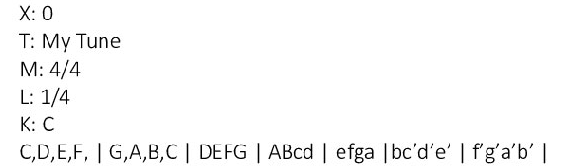
\includegraphics[width=3.25cm,height=0.96cm,keepaspectratio]{intro/abc_user.png}};
\node[font=\scriptsize] at (7.35,0.75) {\textit{ABC}-нотация};
\node[draw=HSEorange, fill=white, thick, rounded corners=5pt,
    align=center, minimum width=3.45cm, minimum height=1.12cm, inner sep=1pt] (midi) at (7.35,0)
    {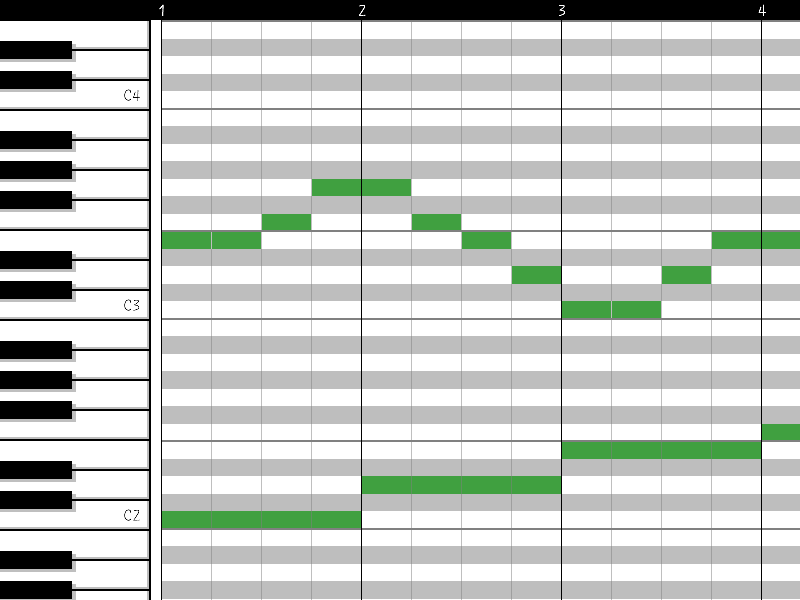
\includegraphics[width=3.05cm,height=0.93cm,keepaspectratio]{intro/midi_piano_roll.png}};
\node[font=\scriptsize] at (7.35,-0.77) {\textit{MIDI}-файл};
\node[draw=HSEred, fill=white, thick, rounded corners=5pt,
    align=center, minimum width=3.45cm, minimum height=1.12cm, inner sep=1pt] (wave) at (7.35,-1.52)
    {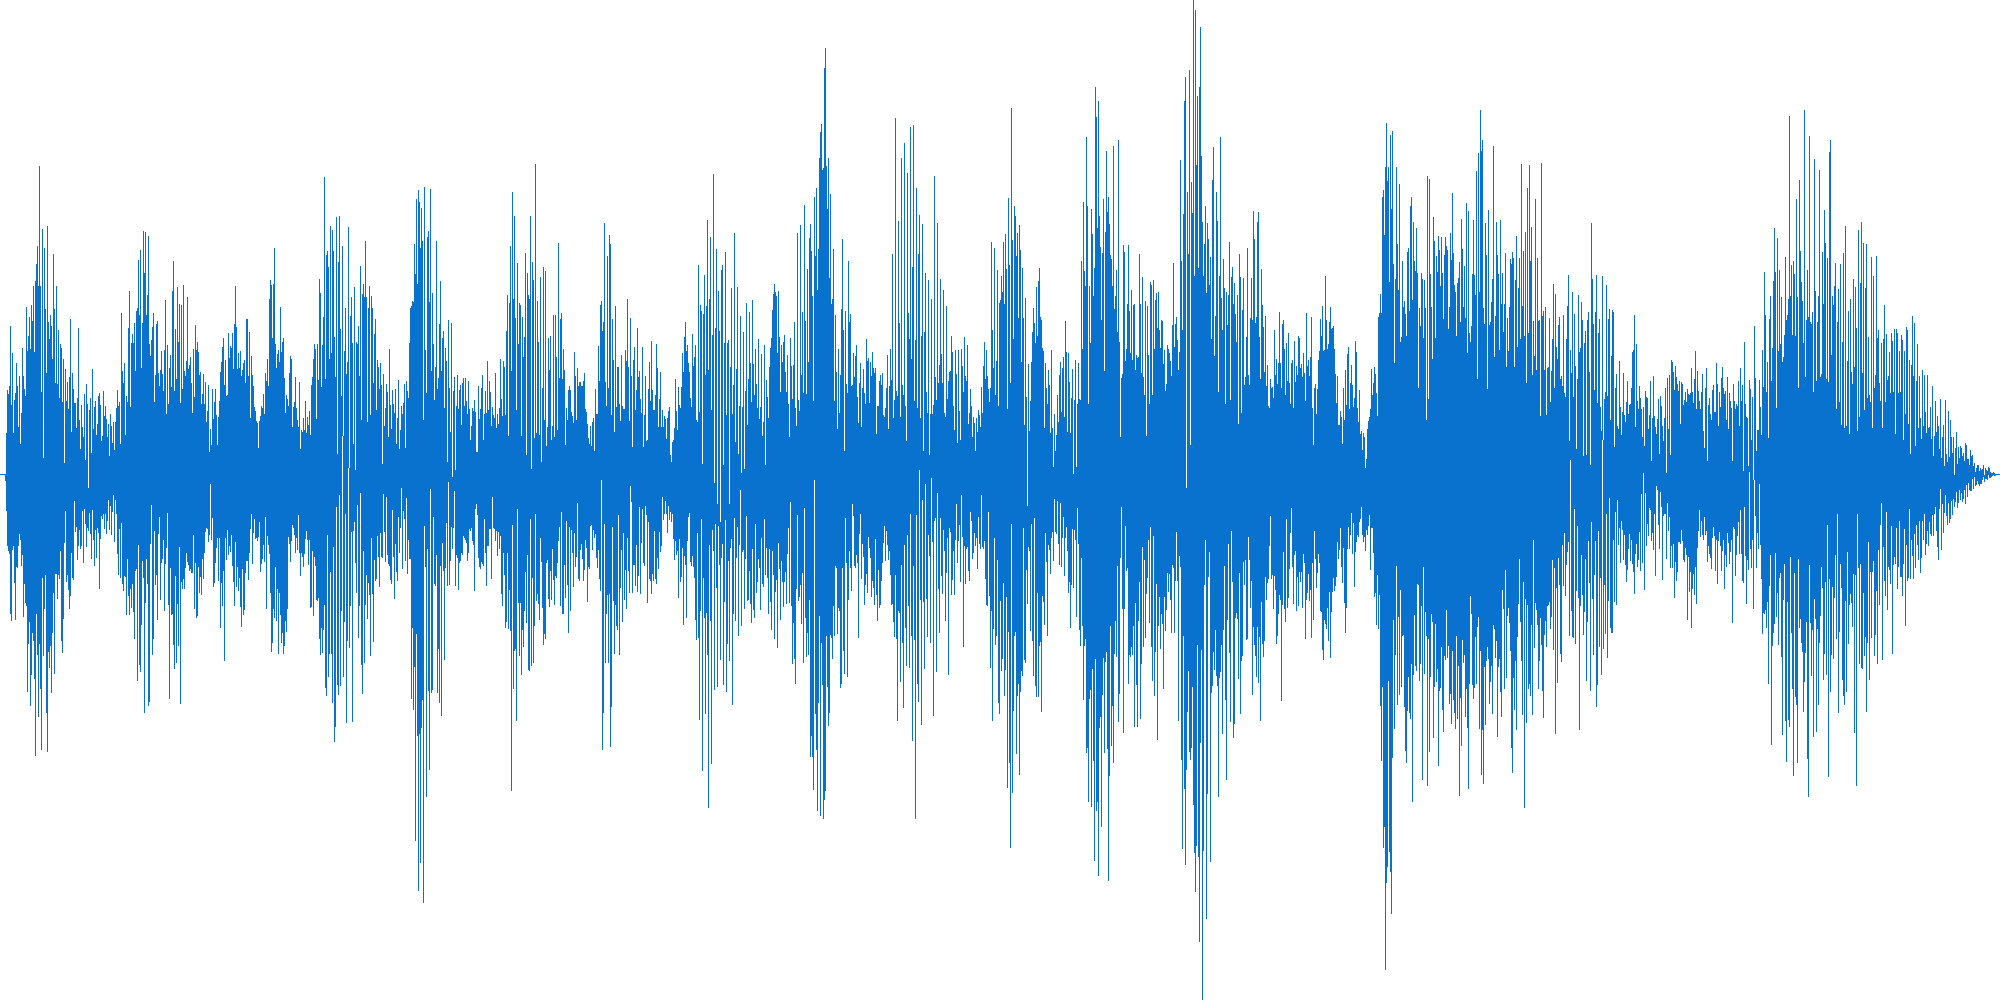
\includegraphics[width=3.25cm,height=0.96cm,keepaspectratio]{intro/waveform_user.png}};
\node[font=\scriptsize] at (7.35,-2.29) {аудиосигнал};
\draw[->, very thick, HSEblue] (prompt.east) -- (model.west);
\draw[->, thick, HSEblue] (model.east) -- (abc.west);
\draw[->, thick, HSEblue] (model.east) -- (midi.west);
\draw[->, thick, HSEblue] (model.east) -- (wave.west);
\end{tikzpicture}

\medskip
\small
Одна музыкальная идея может быть представлена как текстовая запись, \textit{MIDI}-файл или готовый звук.
В работе нас интересует именно \textit{MIDI}.
\end{frame}

\begin{frame}
\frametitle{Введение: Сложность задачи}
\small
\begin{columns}[T,totalwidth=\textwidth]
\column{0.47\textwidth}
\centering
\begin{tikzpicture}[x=1cm,y=1cm]
\node[draw=HSEblue, fill=HSEblue!9, rounded corners=5pt,
    minimum width=1.0cm, minimum height=0.7cm] (t1) at (0,0) {$y_1$};
\node[draw=HSEblue, fill=HSEblue!9, rounded corners=5pt,
    minimum width=1.0cm, minimum height=0.7cm] (t2) at (1.35,0) {$y_2$};
\node[draw=HSEblue, fill=HSEblue!9, rounded corners=5pt,
    minimum width=1.0cm, minimum height=0.7cm] (t3) at (2.7,0) {$y_3$};
\node[minimum width=1.0cm, minimum height=0.7cm] (dots) at (4.05,0) {$\ldots$};
\node[draw=HSEblue, fill=HSEblue!9, rounded corners=5pt,
    minimum width=1.0cm, minimum height=0.7cm] (tn) at (5.4,0) {$y_T$};
\draw[->, thick, HSEblue] (t1) -- (t2);
\draw[->, thick, HSEblue] (t2) -- (t3);
\draw[->, thick, HSEblue] (t3) -- (dots);
\draw[->, thick, HSEblue] (dots) -- (tn);
\node[align=center, font=\scriptsize] at (2.7,-0.85)
    {модель выбирает следующий токен\\по локальному контексту};
\end{tikzpicture}

\column{0.5\textwidth}
\begin{itemize}
    \item Цельность музыки задаётся не одним токеном, а всей последовательностью.
    \item Важны форма, ритм, гармония, инструменты и соответствие текстовому запросу.
    \item При обучении ``предсказывать следующий токен'' часть общего музыкального сигнала теряется.
\end{itemize}
\end{columns}

\medskip
\begin{alertblock}{Цель работы}
Оценивать уже сгенерированный \textit{MIDI}-фрагмент и использовать этот сигнал для дообучения модели методами обучения с подкреплением.
\end{alertblock}
\end{frame}


\begin{frame}
\frametitle{Введение: Схема дообучения модели}
\small
\centering
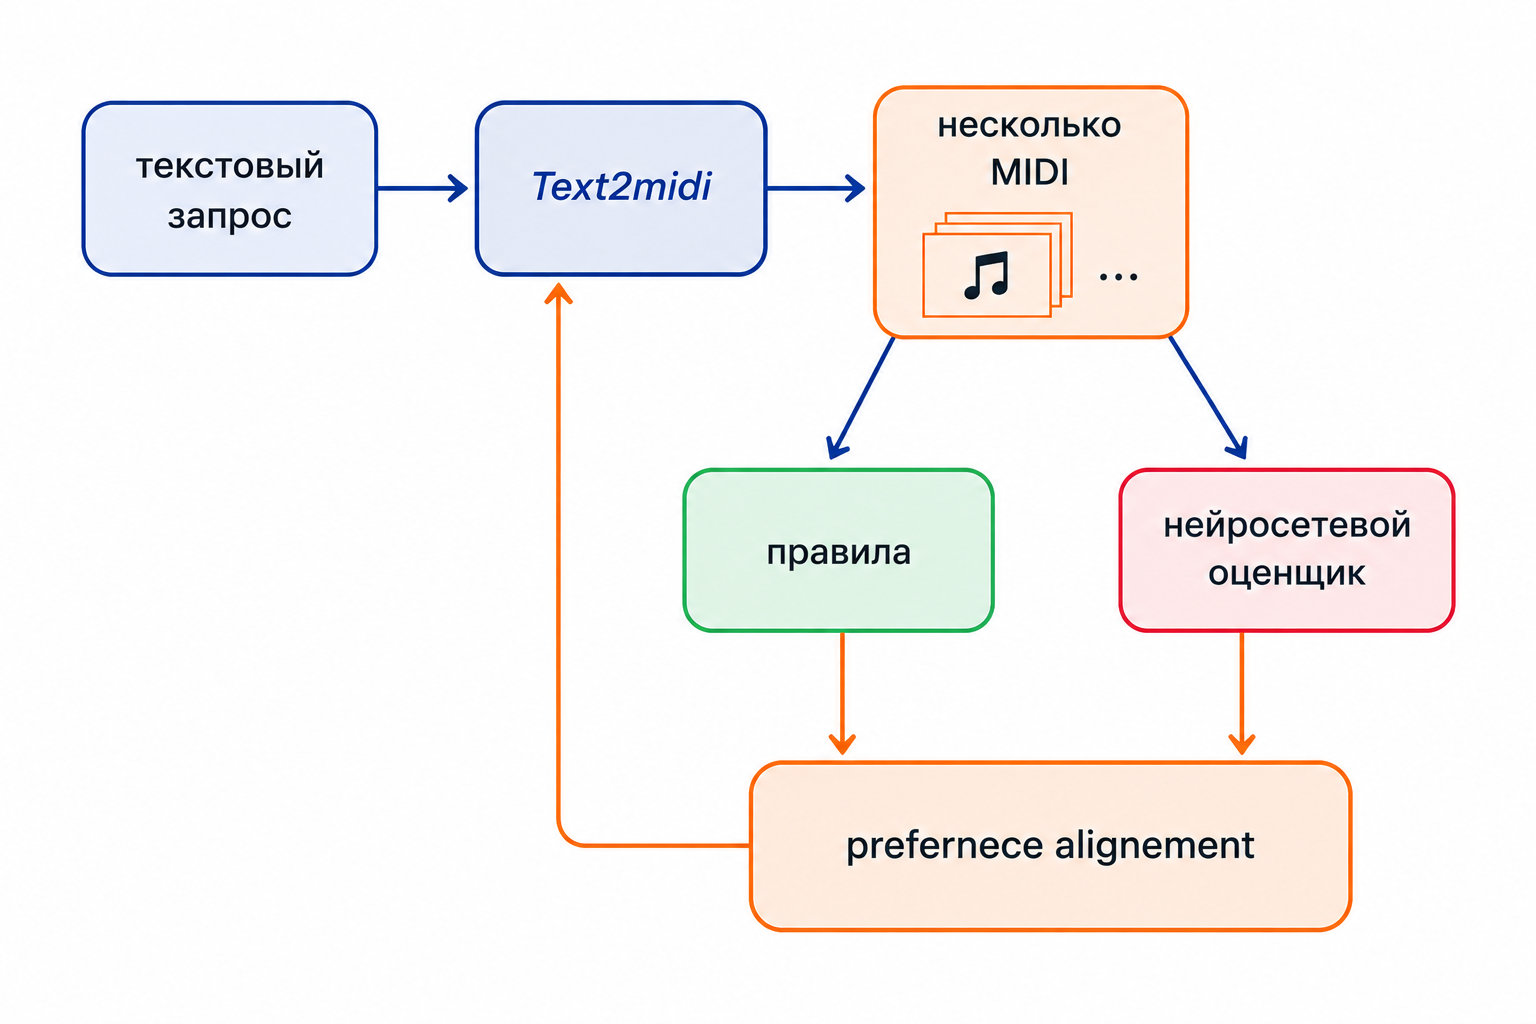
\includegraphics[width=0.96\textwidth,height=0.66\textheight,keepaspectratio]{intro_pic.png}

\vspace{0.08cm}
\footnotesize
\begin{itemize}
    \item \textit{Text2midi} по текстовому запросу порождает несколько кандидатов \textit{MIDI}.
    \item Модель может оценивать кандидаты, например, по правилам и с помощью нейросетевого оценщика.
    \item Для дообучения по внешней оценке можно рассматривать \textit{DPO}, \textit{PPO} и \textit{GRPO}.
\end{itemize}
\end{frame}

\begin{frame}
\frametitle{Обзор литературы: внешняя оценка качества}
\begin{itemize}
    \item В ряде работ музыкальный результат оценивается не по токенам, а по внешнему сигналу качества.
    \item \textit{RL-Duet} использует награду за согласованность с партией второго исполнителя.
    \item \textit{MusicRL} опирается на попарные сравнения и внешний оценщик музыкального качества.
    \item Работа Kumar et al. показывает: чтобы дообучение работало, сигнал оценки должен быть достаточно информативным.
    \item \textit{Text2midi-InferAlign} применяет награду при выборе кандидатов; в нашей работе похожий сигнал переносится в дообучение.
\end{itemize}

\litrefs{RL-Duet: Jiang et al., 2020; MusicRL: Cideron et al., 2024; Kumar et al., 2026; Text2midi-InferAlign: Roy et al., 2025.}
\end{frame}
\begin{frame}
\frametitle{Распределение работы}
\small
\begin{columns}[T,totalwidth=\textwidth]
\column{0.48\textwidth}
\begin{block}{Александр Александрович Вальсамакин}
\begin{itemize}
    \item Выбор и подготовка данных для графового критика.
    \item Обучение и анализ нейросетевого оценщика.
    \item Эксперименты с графовым представлением музыкальных данных.
\end{itemize}
\end{block}

\column{0.48\textwidth}
\begin{block}{Даниил Григорьевич Удалов}
\begin{itemize}
    \item GRPO-дообучение \textit{Text2midi}-модели.
    \item Формализация правил и расчёт наград.
    \item Внедрение критика в схему RL-дообучения.
\end{itemize}
\end{block}
\end{columns}
\end{frame}

\begin{frame}
\frametitle{GNN Critic}
\framesubtitle{HookTheory Dataset}
\vspace{0.2cm}
	 \begin{columns}[c,totalwidth=\textwidth]
	 \column{0.42\textwidth}
		{\fontsize{15}{19}\selectfont
		\textbf{Всего песен:} 26 178\\[0.25cm]
		\textbf{Количество уникальных}\\
		\textbf{исполнителей:} 6 207\\[0.25cm]
		\textbf{Всего нот:} 1 338 346\\[0.25cm]
		\textbf{Всего аккордов:} 449 072}
		\column{0.58\textwidth}
		\begin{center}
			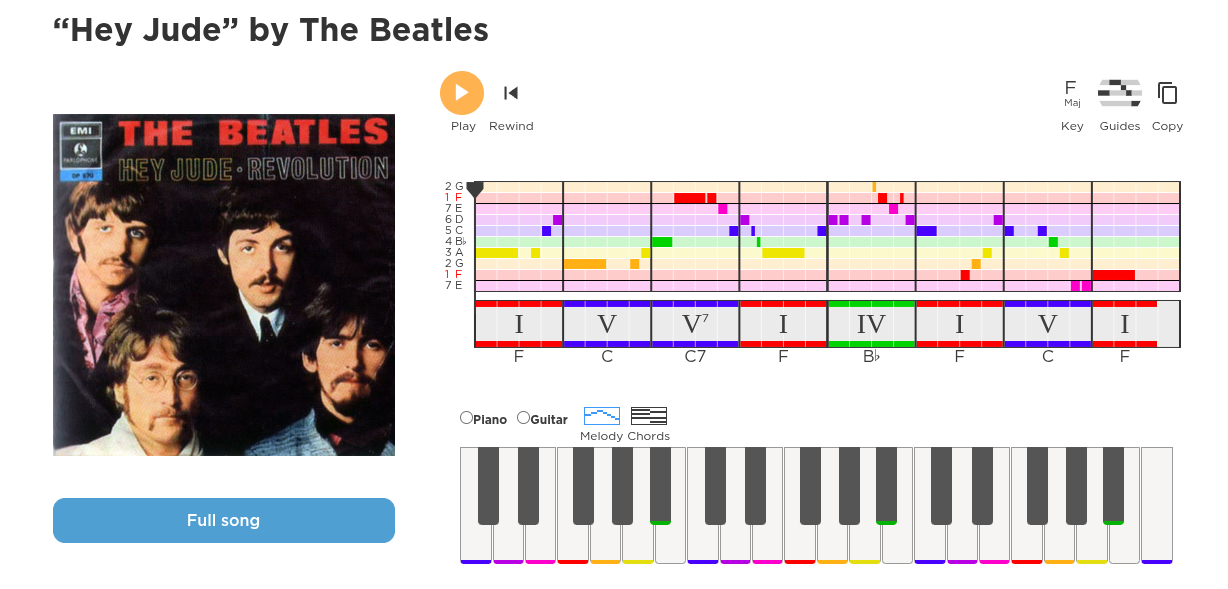
\includegraphics[width=\columnwidth,height=0.56\textheight,keepaspectratio]{image1}\\[0.12cm]
			{\fontsize{14}{17}\selectfont \href{https://www.hooktheory.com/}{HookTheory.com}}
		\end{center}
	\end{columns}
\end{frame}

\begin{frame}
\frametitle{GNN Critic}
\framesubtitle{HookTheory Dataset}
\vspace{0.05cm}
\definecolor{ChordInversion}{RGB}{105,105,105}
\definecolor{ChordAlteration}{RGB}{160,55,55}
\definecolor{ChordOmit}{RGB}{105,65,150}
\definecolor{ChordBorrowed}{RGB}{0,120,120}
\definecolor{ChordApplied}{RGB}{0,115,170}
	 \begin{columns}[T,totalwidth=\textwidth]
	 \column{0.62\textwidth}
		{\fontsize{12.5}{16}\selectfont\raggedright
		\textbf{Каждый клип --- JSON-объект типа:}\\[0.25cm]
		\begin{itemize}
			\setlength{\itemsep}{0.2cm}
			\item \texttt{meta}: \texttt{split}, \texttt{key}, \texttt{tempo}, \texttt{meter}
			\item \texttt{[melody]}: \texttt{beat}, \texttt{duration}, \texttt{scale}, \texttt{degree}, \texttt{octave}, \texttt{rest flag}
			\item \texttt{[chords]}: \texttt{beat}, \texttt{duration}, \textcolor{HSEblue}{\texttt{root}}, \textcolor{HSEgreen}{\texttt{type}}, \textcolor{ChordInversion}{\texttt{inversion}}, \textcolor{ChordApplied}{\texttt{applied}}, \textcolor{HSEorange}{\texttt{adds}}, \textcolor{ChordOmit}{\texttt{omits}}, \textcolor{ChordAlteration}{\texttt{alterations}}, \texttt{suspensions}, \textcolor{ChordBorrowed}{\texttt{borrowed}}, \texttt{rest flag}
		\end{itemize}
		}
		\column{0.38\textwidth}
		\begin{center}
			{\fontsize{28}{34}\selectfont
			\textcolor{HSEblue}{C}%
			\textcolor{HSEgreen}{maj7}%
			\textcolor{HSEorange}{add9}}\\[0.28cm]
			{\fontsize{28}{34}\selectfont
			\textcolor{HSEblue}{A}%
			\textcolor{HSEred}{sus4}}\\[0.28cm]
			{\fontsize{28}{34}\selectfont
			\textcolor{HSEblue}{D}%
			\textcolor{HSEgreen}{7}%
			\textcolor{ChordApplied}{/V}}\\[0.45cm]
			{\fontsize{10}{12}\selectfont
			\textcolor{HSEblue}{root}\quad
			\textcolor{HSEgreen}{type}\quad
			\textcolor{HSEorange}{adds}\quad
			\textcolor{HSEred}{suspensions}\\[0.08cm]
			\textcolor{ChordApplied}{applied}}
		\end{center}
	\end{columns}
\end{frame}

\begin{frame}
\frametitle{GNN Critic}
\framesubtitle{Графовое представление данных}
\vspace{0.05cm}
	 \begin{columns}[c,totalwidth=\textwidth]
	 \column{0.5\textwidth}
		\begin{center}
			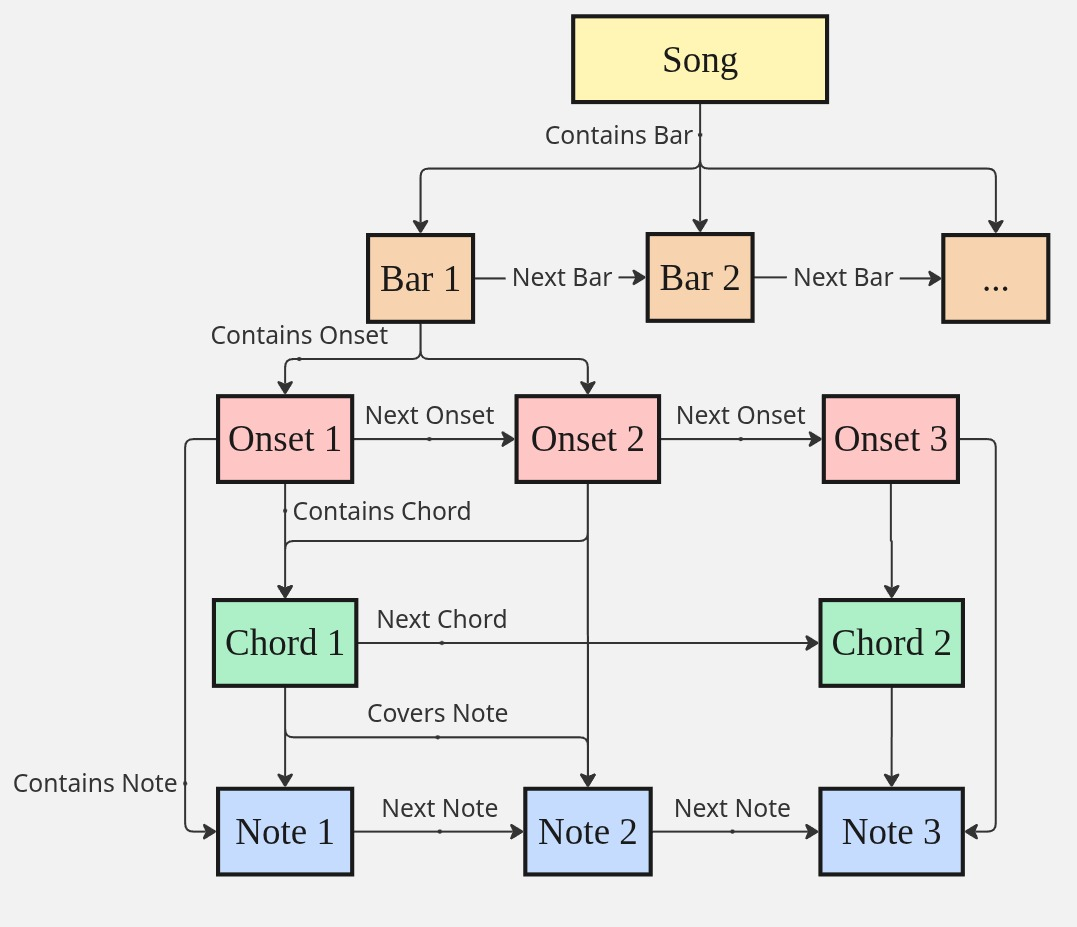
\includegraphics[width=0.96\columnwidth,height=0.63\textheight,keepaspectratio]{graph_hierarchy_edges.jpg}\\[0.12cm]
			{\fontsize{10}{12}\selectfont \textbf{Схема иерархии и типов связей}}
		\end{center}
		\column{0.5\textwidth}
		\begin{center}
			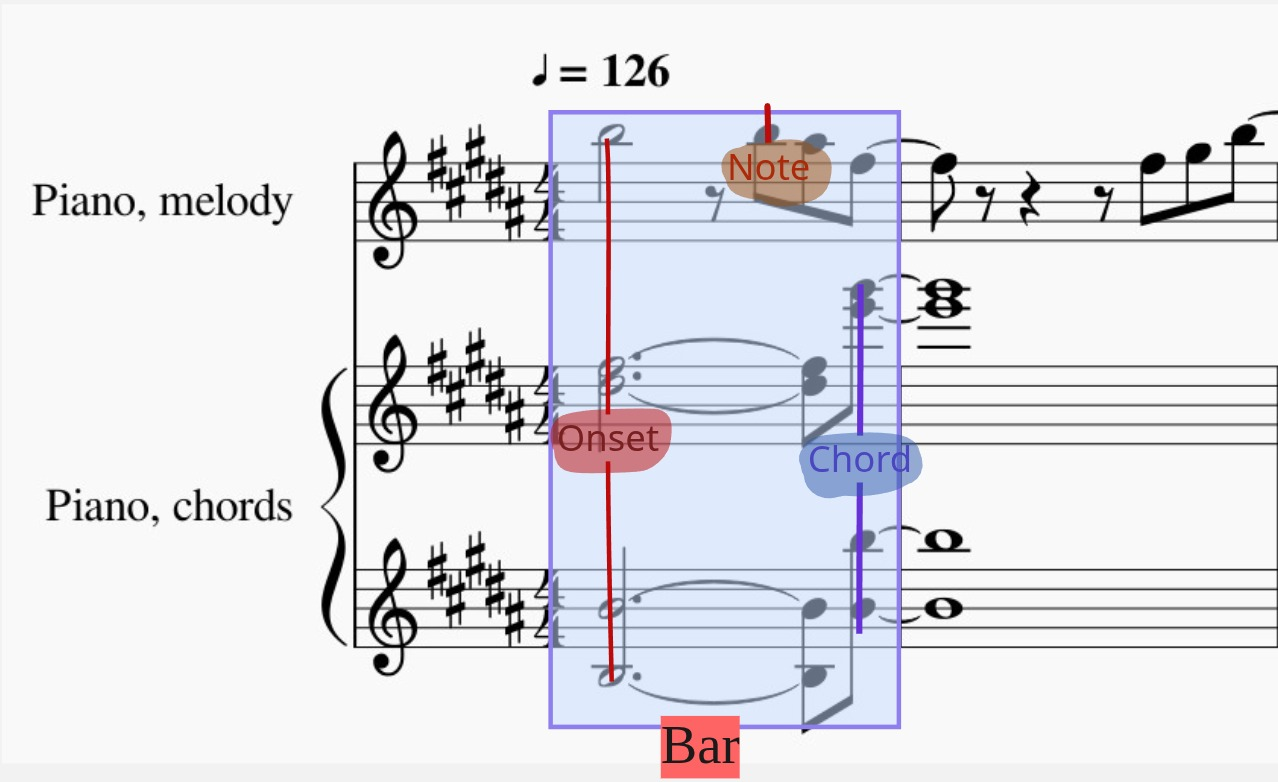
\includegraphics[width=0.96\columnwidth,height=0.63\textheight,keepaspectratio]{graph_hierarchy_score.jpg}\\[0.12cm]
			{\fontsize{10}{12}\selectfont \textbf{Иерархия в формате нотной записи}}
		\end{center}
	\end{columns}
\end{frame}

\begin{frame}
\frametitle{GNN Critic}
\framesubtitle{Пример искажений треков}
\begin{center}
	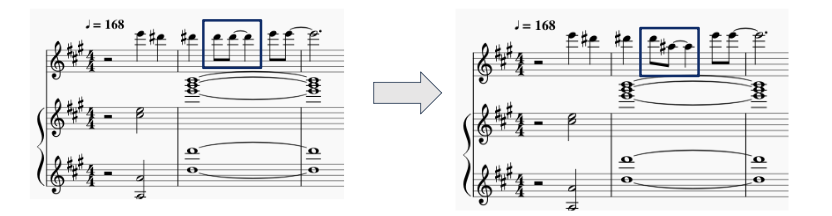
\includegraphics[width=0.95\textwidth,height=0.38\textheight,keepaspectratio]{Screenshot From 2026-05-19 15-45-20.png}\\[0.12cm]
	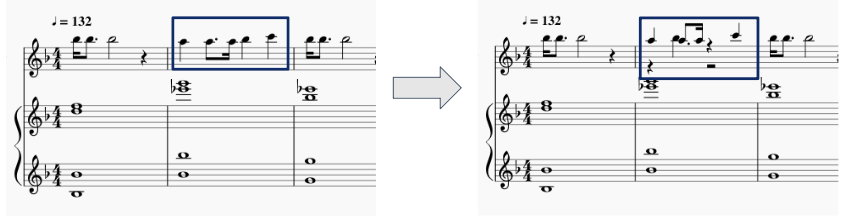
\includegraphics[width=0.95\textwidth,height=0.38\textheight,keepaspectratio]{Screenshot From 2026-05-19 15-45-47.png}\\[0.03cm]
	{\fontsize{10}{12}\selectfont \textbf{Нотная запись до и после искажений}}
\end{center}
\end{frame}

\begin{frame}
\frametitle{GNN Critic}
\framesubtitle{Схема обучения графового критика}
\begin{columns}[c,totalwidth=\textwidth]
	\column{0.24\textwidth}
	{\fontsize{10}{9.6}\selectfont\raggedright
	$\mathcal{G}$ -- исходный граф
	\\[0.15cm]
	$\widetilde{\mathcal{G}}$ -- искаженный граф
	\\[0.15cm]
	Модель обучается выполнять условие:
	\[
	\begin{gathered}
	s_\theta(\mathcal{G}) > s_\theta(\widetilde{\mathcal{G}})
	\end{gathered}
	\]
	}
	\column{0.76\textwidth}
	\centering
	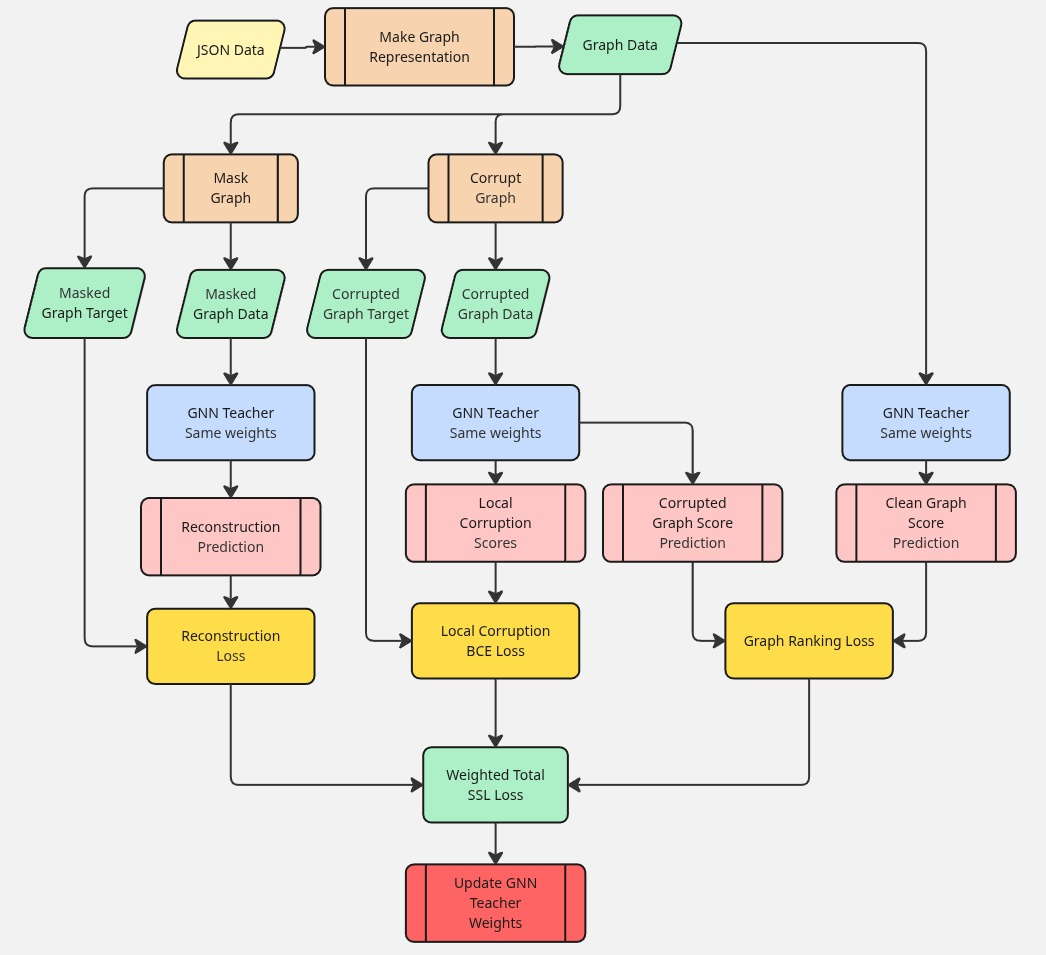
\includegraphics[width=0.8\columnwidth,height=0.72\textheight]{teacher_training_scheme.jpg}\\[0.08cm]
		{\fontsize{10}{12}\selectfont \textbf{Схема обучения графового критика}}
	\end{columns}
\end{frame}

\begin{frame}
\frametitle{GNN Critic}
\framesubtitle{Схема применения графового критика}
\centering
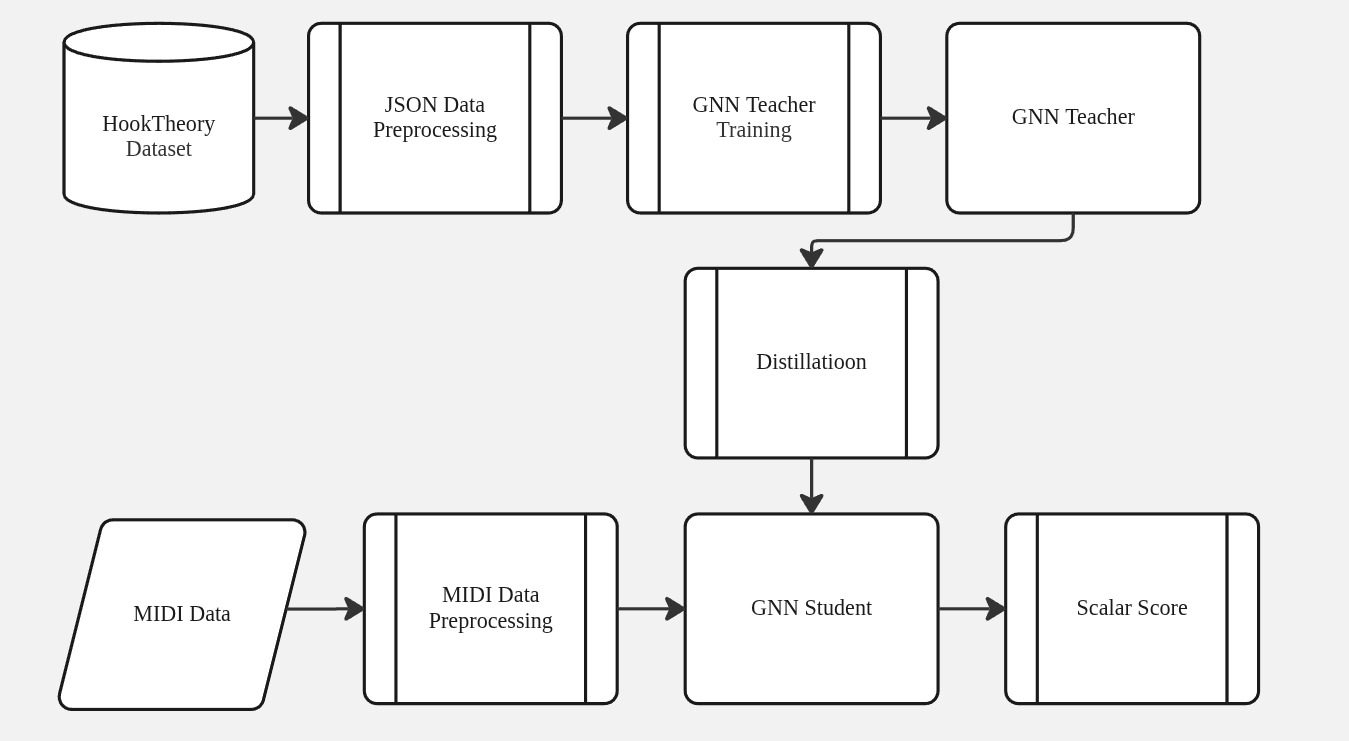
\includegraphics[width=0.9\textwidth,height=0.68\textheight,keepaspectratio]{GNNCriticScheme.jpg}\par
\vspace{0.08cm}
{\fontsize{10}{12}\selectfont \textbf{Схема применения графового критика}}
\end{frame}

\begin{frame}
\frametitle{GNN Critic}
\framesubtitle{Схема обучения графового учителя}
\begin{columns}[c,totalwidth=\textwidth]
	\column{0.24\textwidth}
	{\fontsize{10}{9.6}\selectfont\raggedright
	$\mathcal{G}$ -- исходный граф
	\\[0.15cm]
	$\widetilde{\mathcal{G}}$ -- искаженный граф
	\\[0.15cm]
	Модель обучается выполнять условие:
	\[
	\begin{gathered}
	s_\theta(\mathcal{G}) > s_\theta(\widetilde{\mathcal{G}})
	\end{gathered}
	\]
	}
	\column{0.76\textwidth}
	\centering
	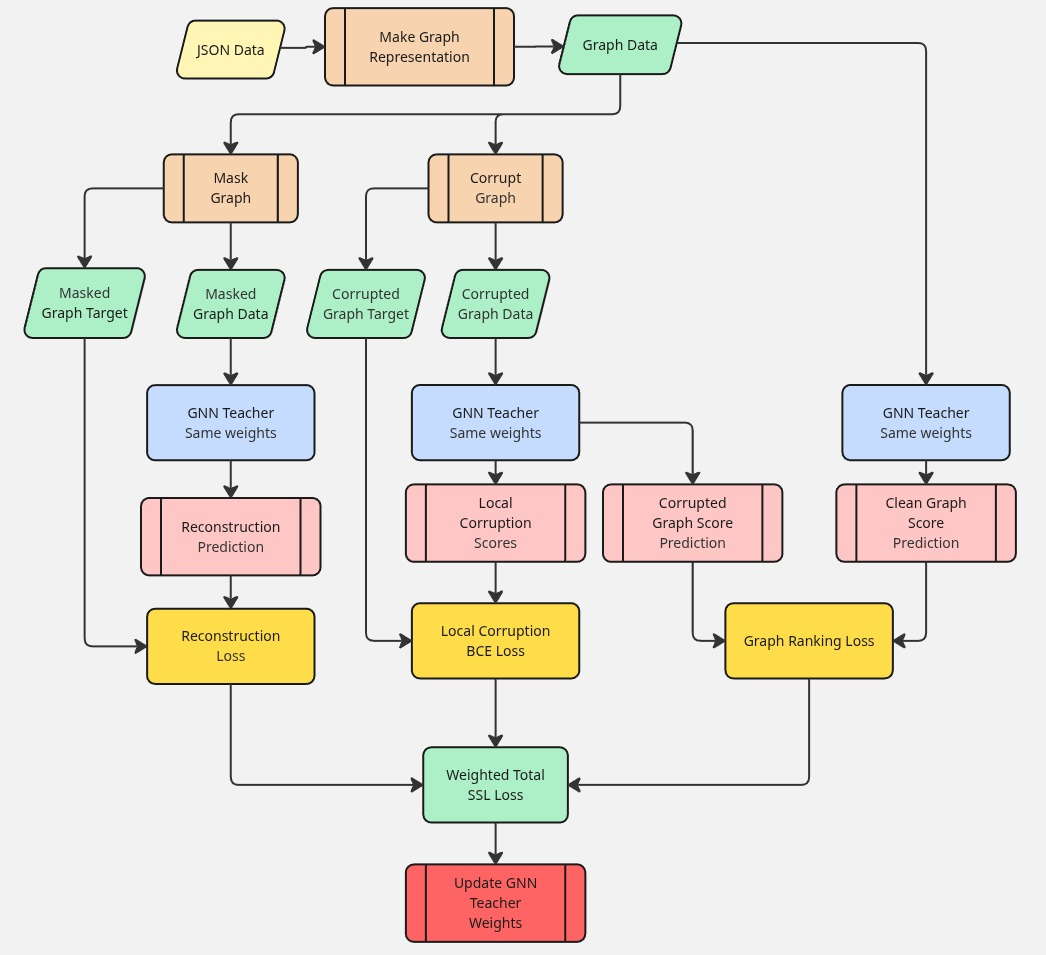
\includegraphics[width=0.8\columnwidth,height=0.72\textheight]{teacher_training_scheme.jpg}\\[0.08cm]
		{\fontsize{10}{12}\selectfont \textbf{Схема обучения графового \crossouttext{критика} учителя}}
	\end{columns}
\end{frame}

\begin{frame}
\frametitle{GNN Critic}
\framesubtitle{Схема обучения графового ученика}
\centering
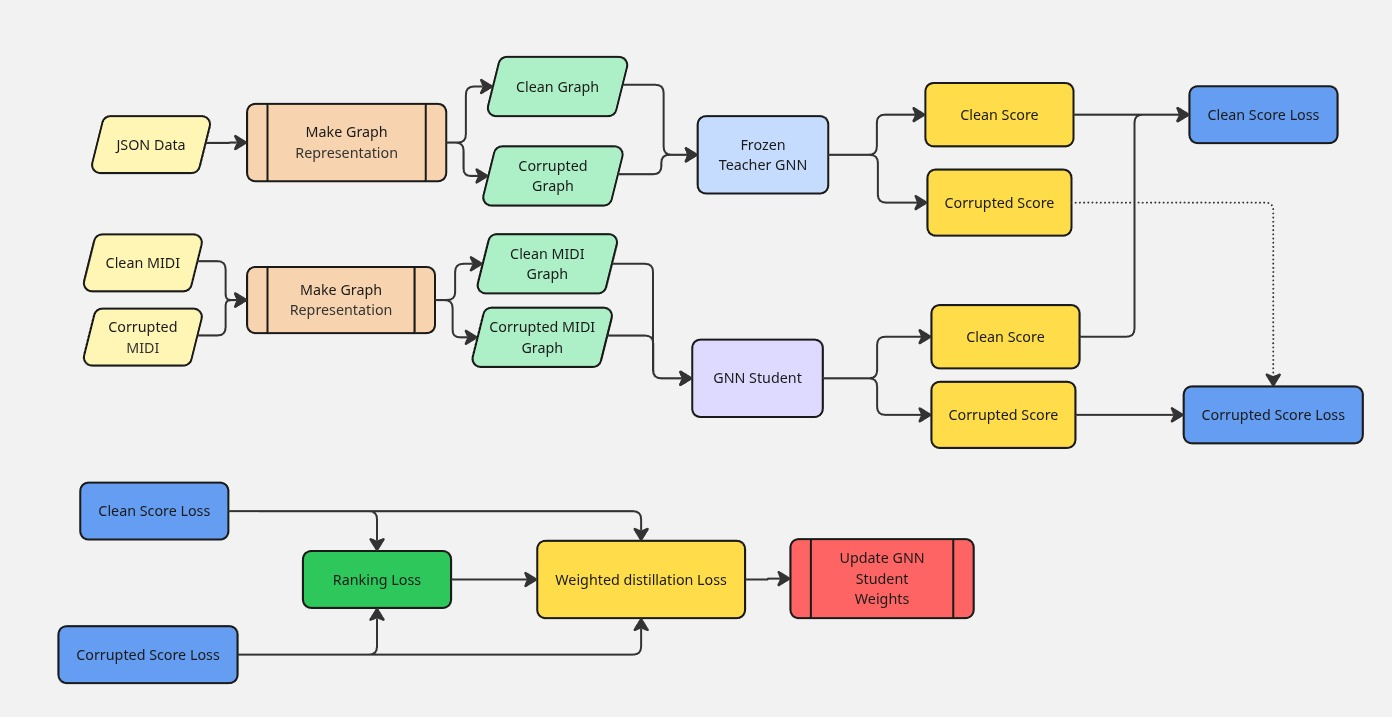
\includegraphics[width=0.9\textwidth,height=0.68\textheight,keepaspectratio]{student_training_scheme.jpg}\par
\vspace{0.08cm}
{\fontsize{10}{12}\selectfont \textbf{Общая схема обучения графового ученика}}
\end{frame}

\begin{frame}
\frametitle{GNN Critic}
\framesubtitle{Механизм определения аккордов из MIDI}
\vspace{-0.05cm}
\definecolor{MidiHeader}{RGB}{222,222,222}
\definecolor{MidiRowA}{RGB}{198,207,230}
\definecolor{MidiRowB}{RGB}{228,232,242}
\begin{center}
	{\large Ноты на входе: \texttt{C - E - G - B}}
\end{center}

\vspace{0.12cm}
\centering
{\fontsize{9}{10.8}\selectfont
\setlength{\tabcolsep}{5pt}
\renewcommand{\arraystretch}{1.35}
\resizebox{0.93\textwidth}{!}{%
\begin{tabular}{>{\raggedright\arraybackslash}p{4.0cm}
	>{\raggedright\arraybackslash}p{5.0cm}
	>{\raggedright\arraybackslash}p{3.8cm}}
\rowcolor{MidiHeader}
\multicolumn{1}{>{\centering\arraybackslash}p{4.0cm}}{Возможная интерпретация} &
\multicolumn{1}{>{\centering\arraybackslash}p{5.0cm}}{Функция} &
\multicolumn{1}{>{\centering\arraybackslash}p{3.8cm}}{Лад / тональный контекст} \\
\rowcolor{MidiRowA}
Cmaj7 & I --- тоника & C Ionian \\
\rowcolor{MidiRowB}
Em($\flat$13) & i --- модальная тоника & E Phrygian \\
\rowcolor{MidiRowA}
G6sus4 (или G(add4,6)) & I с суспензией / тоническое зависание & G Ionian \\
\rowcolor{MidiRowB}
Cmaj7 & III --- медиантовая окраска & A melodic minor \\
\rowcolor{MidiRowA}
B$\varnothing$(add$\flat$9) (условная неполная трактовка) & i$\varnothing$ --- локрийская тоника & B Locrian \\
\rowcolor{MidiRowB}
Cmaj7 & V --- доминантовая ступень без классического доминантового напряжения & F Lydian \\
\end{tabular}
}
}
\end{frame}

\begin{frame}
\frametitle{GNN Critic}
\framesubtitle{Аккордовый оценщик}
\vspace{0.2cm}
{\fontsize{15}{19}\selectfont
Аккордовый оценщик выбирает кандидата с наибольшим количеством очков соответствия, которые считаются как:
}
\[
q(c, P_w)
=
q_{+}(c, P_w)
-
q_{-}(c, P_w),
\]
\vspace{0.1cm}
{\fontsize{13}{17}\selectfont
\begin{itemize}
	\setlength{\itemsep}{0.18cm}
	\item $P_w$ --- наблюдаемые ноты;
	\item $c$ --- аккордовый кандидат;
	\item $q_{+}$ --- \hyperlink{positive-score}{положительный вклад} объяснённых признаков;
	\item $q_{-}$ --- \hyperlink{negative-score}{штрафы за несоответствия}.
\end{itemize}
}
\end{frame}



\begin{frame}
\frametitle{GNN Critic}
\framesubtitle{Сравнение механизмов искажения}
\begin{table}
\centering
\scriptsize
{\normalsize Сравнение случайных и теоретически обоснованных искажений}\\[0.25cm]
\label{tab:1}
\resizebox{0.68\textwidth}{!}{%
\begin{tabular}{@{}lllll@{}}
\toprule
\textit{Corruption family} & \textit{Pooling} & \textit{Best rank acc} $\uparrow$ \\
\midrule
\textit{Theory-aware} & \textit{mean\_max} & \textbf{1.0000} \\
\textit{Graph} & \textit{mean\_max}  & 0.8750 \\
\bottomrule
\end{tabular}%
}
\end{table}
\end{frame}

\begin{frame}
\frametitle{GNN Critic}
\framesubtitle{Обзор обобщающей способности критика}
\begin{table}[htbp]
{\Large Проверка обобщения teacher-модели на OOD-corruptions}\\[0.25cm]
\label{tab:ood-corruption-groups}
\centering
\small
\setlength{\tabcolsep}{4pt}
\renewcommand{\arraystretch}{1.25}
\begin{tabular}{@{}p{3.5cm}p{1.7cm}p{1cm}p{6.2cm}@{}}
\toprule
\textit{Group} & \textit{Mean gap} & \textit{Global RankAcc} & \textit{Interpretation} \\
\midrule
\textit{Harmful OOD corruptions} & 0.6649 & 0.5504 & Новые вредные искажения в среднем понижают \textit{score} \\
\textit{Benign transformations} & 0.0110 & 0.5012 & Безвредные преобразования почти не создают систематический штраф \\
\bottomrule
\end{tabular}
\end{table}
\end{frame}

\begin{frame}
\frametitle{GNN Critic}
\framesubtitle{Staged training}
\begin{table}[htbp]
\centering
{\normalsize\textit{Staged training}}\\[0.25cm]
\label{tab:3}
\scriptsize
\resizebox{\textwidth}{!}{%
\begin{tabular}{@{}llllllllll@{}}
\toprule
\textit{Training mode} & \textit{Best IntraAcc} $\uparrow$ & \textit{Best InterAcc} $\uparrow$ & \textit{BinaryAcc} $\uparrow$ \\
\midrule
\textit{MLM} $\to$ \textit{corruption}   & \textbf{0.9118} & \textbf{0.8994} & 0.7486 \\
\textit{Corruption from scratch} & 0.9007 & 0.8962 & \textbf{0.7489} \\
\bottomrule
\end{tabular}%
}
\end{table}
\MetricLegend
\end{frame}

\begin{frame}
\frametitle{GNN Critic}
\framesubtitle{Feature ablation}
\begin{table}[htbp]
\centering
{\normalsize\textit{Feature ablation}: \textit{dynamic weighting}, \textit{HGT} и \textit{learned logit fusion}}\\[0.25cm]
\label{tab:4}
\scriptsize
\resizebox{\textwidth}{!}{%
\begin{tabular}{@{}llllllllll@{}}
\toprule
\textit{Variant} & \textit{Backbone} & \textit{Dynamic weights} & \textit{Logit fusion} & \textit{Best IntraAcc} $\uparrow$ & \textit{Best InterAcc} $\uparrow$ & \textit{BinaryAcc} $\uparrow$ \\
\midrule
\textit{Baseline} & \textit{SAGE} & \textit{no} & \textit{no} & 0.8547 & 0.8472 & 0.7668 \\
\textit{HGT} & \textit{HGT} & \textit{no} & \textit{no}  & 0.8410 & 0.8409 & 0.7537 \\
\textit{Dynamic weights} & \textit{SAGE} & \textit{yes} & \textit{no}  & 0.8530 & \textbf{0.8494} & \textbf{0.7731} \\
\textit{Learned logit fusion} & \textit{SAGE} & \textit{no} & \textit{yes} & 0.8408 & \textbf{0.8523} & \textbf{0.7761} \\
\bottomrule
\end{tabular}%
}
\end{table}
\MetricLegend
{\scriptsize\textit{Источники:} \href{https://arxiv.org/html/2509.06654v1}{\textit{AnalysisGNN: Unified Music Analysis with Graph Neural Networks}: Karystinaios et al., 2025.}}
\end{frame}

\begin{frame}
\frametitle{GNN Critic}
\framesubtitle{Финальная teacher-конфигурация}
\begin{table}[htbp]
\centering
{\normalsize Финальная \textit{teacher}-конфигурация}\\[0.25cm]
\label{tab:5}
\scriptsize
\resizebox{\textwidth}{!}{%
\begin{tabular}{@{}llllllllllll@{}}
\toprule
\textit{Backbone} & \textit{Dynamic weights} & \textit{Logit fusion} & \textit{Hidden / layers} & \textit{Pooling} & \textit{Local context} & \textit{MLM / corr epochs} & \textit{Best IntraAcc} $\uparrow$ & \textit{Best InterAcc} $\uparrow$ & \textit{BinaryAcc} $\uparrow$ \\
\midrule
\textit{SAGE} & \textit{yes} & \textit{yes} & 256 / 4 & \textit{mean\_max} & \textit{attention} & 30 / 39 & \textbf{0.9275} & \textbf{0.9250} & \textbf{0.8456} \\
\bottomrule
\end{tabular}%
}
\end{table}
\MetricLegend
\end{frame}

\begin{frame}
\frametitle{GNN Critic}
\framesubtitle{Scoring для восстановления аккордов из MIDI}
\begin{table}[htbp]
\centering
{\normalsize Сравнение ручного и обучаемого \textit{scoring} для восстановления аккордов из \textit{MIDI}}\\[0.25cm]
\label{tab:chord-prediction-scoring}
\scriptsize
\resizebox{\textwidth}{!}{%
\begin{tabular}{@{}lrrrrrrr@{}}
\toprule
\textit{Scoring} & \textit{Top-1 exact} $\uparrow$ & \textit{Top-5 contains GT} $\uparrow$ & \textit{Root acc} $\uparrow$ & \textit{Type acc} $\uparrow$ & \textit{Root+Type acc} $\uparrow$ & \textit{Mode acc} $\uparrow$ & \textit{Inversion acc} $\uparrow$ \\
\midrule
\textit{Learned weights} & \textbf{0.9216} & \textbf{0.9907} & \textbf{0.9753} & \textbf{0.9864} & \textbf{0.9690} & \textbf{0.9324} & \textbf{0.9811} \\
\textit{Manual} & 0.7641 & 0.9184 & 0.9249 & 0.8368 & 0.8147 & 0.9061 & 0.9213 \\
\bottomrule
\end{tabular}%
}
\end{table}
\end{frame}

\begin{frame}
\frametitle{GNN Critic}
\framesubtitle{Качество восстановления аккордов по типам}
\begin{table}[htbp]
\centering
{\normalsize Качество восстановления аккордов по типам}\\[0.25cm]
\label{tab:chord-type-accuracy}
\footnotesize
\begin{tabular}{@{}lrr@{}}
\toprule
\textit{Type} & \textit{Manual weights} $\uparrow$ & \textit{Learned weights} $\uparrow$ \\
\midrule
\textit{triad / 5} & 0.915 & \textbf{0.938} \\
\textit{seventh / 7} & 0.227 & \textbf{0.867} \\
\textit{ninth / 9} & 0.000 & \textbf{0.850} \\
\textit{eleventh / 11} & 0.000 & \textbf{0.886} \\
\textit{thirteenth / 13} & 0.000 & \textbf{0.089} \\
\bottomrule
\end{tabular}
\end{table}
\end{frame}

\begin{frame}
\frametitle{GNN Critic}
\framesubtitle{Промежуточная дистилляция}
\vspace{-0.28cm}
{\fontsize{9.6}{11}\selectfont
\[
\begin{aligned}
\mathcal{L}
={}&
\lambda_s \mathcal{L}_{score}
+
\lambda_r \mathcal{L}_{rank}
+
\lambda_m \mathcal{L}_{margin}
+
\lambda_g \mathcal{L}_{graph}
+
\lambda_t \mathcal{L}_{type}
+
\lambda_l \mathcal{L}_{local}.
\end{aligned}
\]
\vspace{-0.35cm}
\begin{columns}[T,totalwidth=\textwidth]
	\column{0.48\textwidth}
	\[
	\mathcal{L}_{graph}
	=
	\left\|
	P_g z_G^{S} - z_G^{T}
	\right\|_2^2
	\]
	\vspace{-0.28cm}
	\[
	\mathcal{L}_{type}
	=
	\sum_{\tau}
	\left\|
	P_\tau z_{\tau}^{S} - z_{\tau}^{T}
	\right\|_2^2
	\]
	\vspace{-0.28cm}
	\[
	\mathcal{L}_{local}
	=
	\left\|
	P_l u^{S} - u^{T}
	\right\|_2^2
	\]
	\column{0.5\textwidth}
	\raggedright
	$z_G^{S}$ и $z_G^{T}$ --- графовые \textit{embeddings} \textit{student}- и \textit{teacher}-моделей.\\[0.08cm]
	$z_{\tau}^{S}$ и $z_{\tau}^{T}$ --- \textit{pooled}-представления по типам вершин.\\[0.08cm]
	$u^{S}$ и $u^{T}$ --- локальные \textit{summary}-признаки.\\[0.08cm]
	Матрицы $P_g$, $P_\tau$, $P_l$ являются \textit{projection adapters}, позволяющими сопоставить пространства \textit{student} и \textit{teacher}.
\end{columns}
}
\end{frame}

\begin{frame}
\frametitle{GNN Critic}
\framesubtitle{Дистилляция промежуточных представлений}
\begin{table}[htbp]
\centering
{\normalsize Влияние дистилляции промежуточных представлений \textit{teacher}-модели}\\[0.25cm]
\label{tab:student-intermediate-ablation}
\scriptsize
\resizebox{\textwidth}{!}{%
\begin{tabular}{@{}lrrrrrr@{}}
\toprule
\textit{Variant} & \textit{Batch rank acc} $\uparrow$ & \textit{Spearman} $\uparrow$ & \textit{Pearson} $\uparrow$ & \textit{MAE} $\downarrow$ & \textit{Score distill loss} $\downarrow$ \\
\midrule
\textit{Intermediate} & \textbf{0.6787} & \textbf{0.4173} & \textbf{0.3588} & \textbf{2.3121} & \textbf{3.7560} \\
\textit{No intermediate} & 0.6111 & 0.2712 & 0.1728 & 2.5432 & 4.2046 \\
\bottomrule
\end{tabular}%
}
\end{table}
{\fontsize{6.9}{7.8}\selectfont
\textit{Batch rank acc} --- доля корректных сравнений между всеми положительными и отрицательными примерами внутри батча.\\[0.03cm]
\textit{Spearman} --- ранговая корреляция между оценками \textit{student} и \textit{teacher}.\\[0.03cm]
\textit{Pearson} --- линейная корреляция между этими оценками.\\[0.03cm]
}
\end{frame}

\begin{frame}
\frametitle{GNN Critic}
\framesubtitle{Финальное сравнение observer-конфигураций}
\begin{table}[htbp]
\centering
{\normalsize Финальное сравнение \textit{observer}-конфигураций}\\[0.25cm]
\label{tab:observer-final-comparison}
\scriptsize
\resizebox{\textwidth}{!}{%
\begin{tabular}{@{}lllrrrrrr@{}}
\toprule
\textit{Observer variant} & \textit{Intermediate losses}  & \textit{Pair rank acc} $\uparrow$ & \textit{Batch rank acc} $\uparrow$ & \textit{Spearman} $\uparrow$ & \textit{Pearson} $\uparrow$ & \textit{MAE} $\downarrow$ \\
\midrule
\textit{Intermediate} &  \textit{yes}  & \textbf{0.8692} & \textbf{0.8464} & 0.6926 & \textbf{0.6873} & 2.0698 \\
\textit{No intermediate} &  \textit{no}  & 0.8509 & 0.8387 & \textbf{0.7135} & 0.6832 & \textbf{1.4717} \\
\bottomrule
\end{tabular}%
}
\end{table}
\end{frame}


\begin{frame}
\frametitle{Постановка задачи генерации MIDI по тексту}
\centering
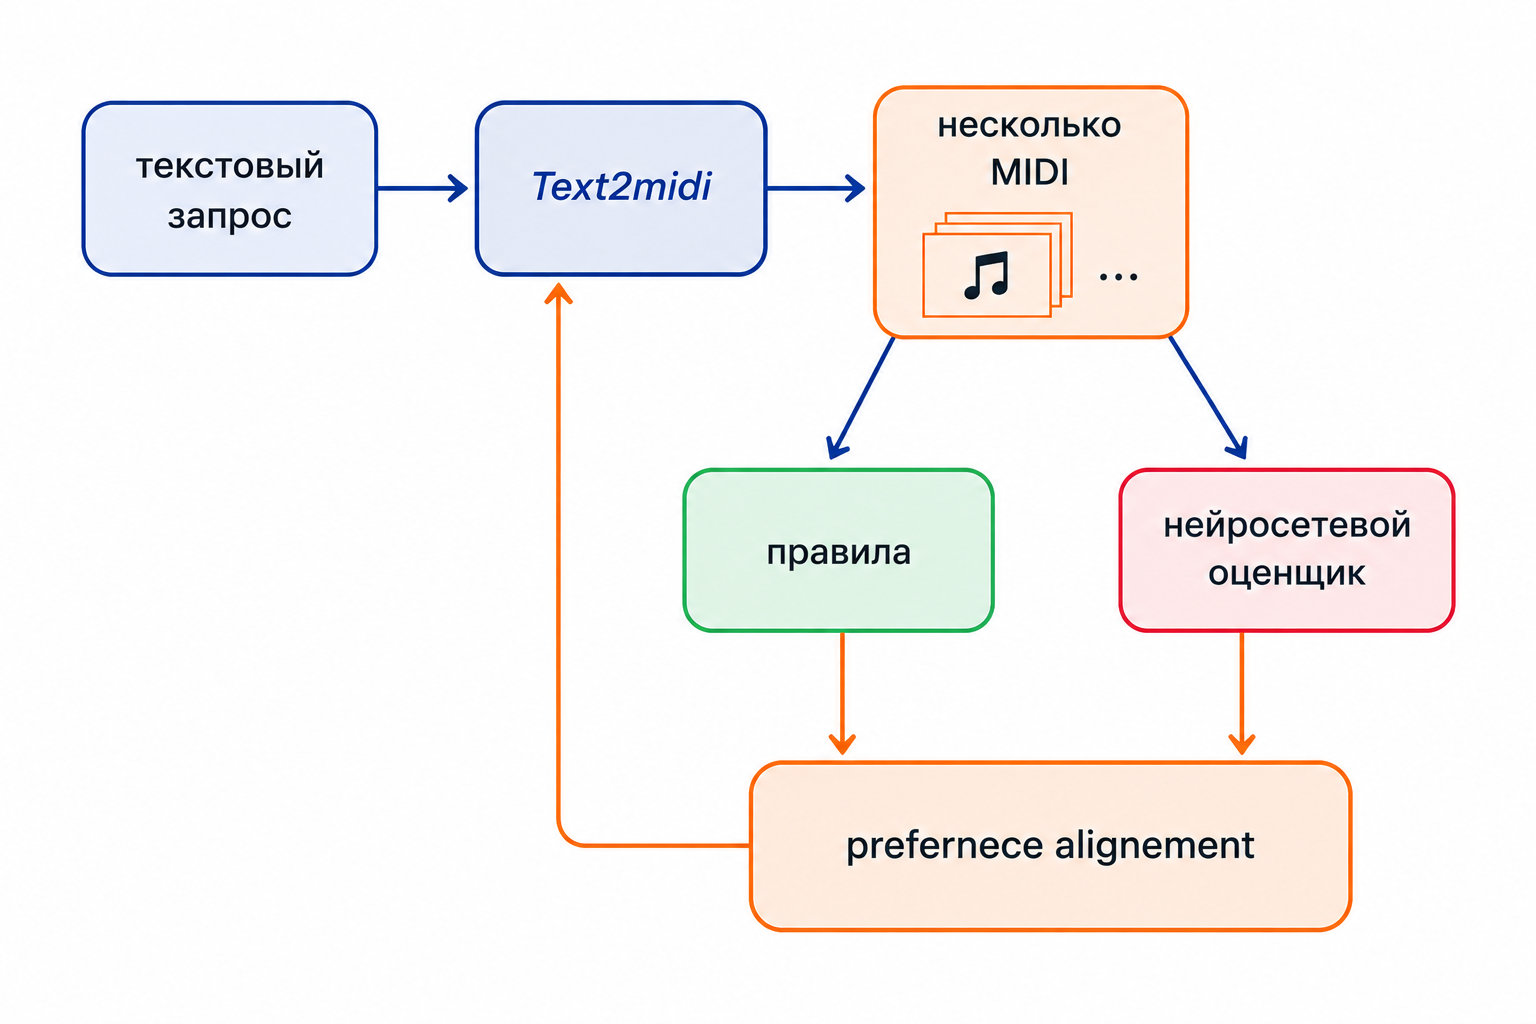
\includegraphics[width=0.9\textwidth,height=0.5\textheight,keepaspectratio]{intro_pic.png}

\vspace{0.1cm}
{\scriptsize
\resizebox{0.92\textwidth}{!}{%
\begin{tabular}{p{0.08\textwidth} p{0.25\textwidth} p{0.57\textwidth}}
\toprule
\textbf{Этап} & \textbf{Операция} & \textbf{Зачем нужна} \\
\midrule
1 & Выбор запроса & Фиксирует текстовое условие для группы кандидатов. \\
2 & Генерация & Модель порождает несколько MIDI-вариантов. \\
3 & Декодирование & Токены переводятся в MIDI-представление. \\
4 & Награда & Правила или критик оценивают готовый фрагмент. \\
5 & Нормировка & Кандидаты сравниваются внутри одной группы. \\
6 & Обновление & GRPO усиливает варианты лучше среднего. \\
\bottomrule
\end{tabular}
}
}
\end{frame}

\begin{frame}
\frametitle{GRPO: преимущество и функция потерь}
\small
\begin{itemize}
    \item Кандидаты сравниваются только внутри одной группы ответов на запрос.
    \item Если награда выше среднего, кандидат усиливается; если ниже --- ослабляется.
\end{itemize}

\vspace{0.05cm}
\begin{columns}[T,totalwidth=\textwidth]
\column{0.46\textwidth}
\[
\bar r=\frac{1}{G}\sum_{j=1}^{G}r_j,
\qquad
\hat{A}_i =
\frac{r_i-\bar r}{s_r+\varepsilon_A}.
\]
\column{0.5\textwidth}
\[
\rho_{i,t}(\theta)=
\frac{\pi_\theta(o_{i,t}\mid q,o_{i,<t})}
{\pi_{\theta_{\mathrm{old}}}(o_{i,t}\mid q,o_{i,<t})}.
\]

\[
\mathcal{L}_{\mathrm{GRPO}}
\sim
-\min\left(
\rho_{i,t}\hat{A}_i,\,
\rho^{\text{огр}}_{i,t}\hat{A}_i
\right)
\;+\;\beta D_{i,t}.
\]
\end{columns}

\begin{itemize}
    \item Отсечение ограничивает слишком резкое обновление, а KL удерживает модель рядом с исходной.
    \item Отдельная модель ценности не требуется.
\end{itemize}
\end{frame}

\begin{frame}
\frametitle{Награды: компоненты на основе правил}
\centering
\begin{tikzpicture}[x=1cm,y=1cm]
\node[draw=HSEorange, fill=HSEorange!16, very thick, rounded corners=8pt,
    align=center, minimum width=3.4cm, minimum height=1.05cm] (center) at (4.6,0.1)
    {награда на основе\\правил};
\node[draw=HSEblue, fill=HSEblue!8, thick, rounded corners=6pt,
    align=center, minimum width=2.5cm, minimum height=0.8cm] (key) at (0.9,1.65)
    {тональность};
\node[draw=HSEblue, fill=HSEblue!8, thick, rounded corners=6pt,
    align=center, minimum width=2.5cm, minimum height=0.8cm] (meter) at (0.9,-1.25)
    {метр};
\node[draw=HSEgreen, fill=HSEgreen!10, thick, rounded corners=6pt,
    align=center, minimum width=2.7cm, minimum height=0.8cm] (dur) at (8.3,1.65)
    {длительность\\и плотность};
\node[draw=HSEgreen, fill=HSEgreen!10, thick, rounded corners=6pt,
    align=center, minimum width=2.7cm, minimum height=0.8cm] (tracks) at (8.3,0.1)
    {дорожки\\и ударные};
\node[draw=HSEred, fill=HSEred!10, thick, rounded corners=6pt,
    align=center, minimum width=2.7cm, minimum height=0.8cm] (valid) at (8.3,-1.45)
    {валидность\\MIDI};
\draw[->, thick, HSEblue] (center) -- (key);
\draw[->, thick, HSEblue] (center) -- (meter);
\draw[->, thick, HSEblue] (center) -- (dur);
\draw[->, thick, HSEblue] (center) -- (tracks);
\draw[->, thick, HSEblue] (center) -- (valid);
\end{tikzpicture}

\vspace{0.12cm}
\begin{itemize}
    \item Правила проверяют, насколько готовый \textit{MIDI}-фрагмент согласован с запросом и не содержит грубых артефактов.
\end{itemize}
\end{frame}

\begin{frame}
\frametitle{Награды: формализация правил}
\small
\begin{columns}[T,totalwidth=\textwidth]
\column{0.48\textwidth}
\begin{block}{Мягкие ограничения}
\[
T(z;l,c,h)=
\begin{cases}
0, & z\le l \ \text{или}\ z\ge h,\\
\frac{z-l}{c-l}, & l<z<c,\\
1, & z=c,\\
\frac{h-z}{h-c}, & c<z<h.
\end{cases}
\]
\end{block}

\column{0.48\textwidth}
\begin{block}{Примеры компонент}
\[
R_{\mathrm{dur}}=T(D;8,64,160)
\]
\[
R_{\mathrm{dens}}=T\left(\frac{|N|}{\max(D,1)};l,c,h\right)
\]
\end{block}
\end{columns}

\medskip
\begin{itemize}
    \item Мягкие функции чаще различают кандидатов внутри группы.
    \item Умеренная плотность снижает риск перегруженных фрагментов.
\end{itemize}
\end{frame}

\begin{frame}
\frametitle{Награды: сигнал критика}
\centering
\begin{tikzpicture}[x=1cm,y=1cm]
\node[draw=HSEblue, fill=HSEblue!8, very thick, rounded corners=8pt,
    align=center, minimum width=2.9cm, minimum height=0.9cm] (midi) at (0.8,0)
    {кандидаты\\\textit{MIDI}};
\node[draw=HSEred, fill=HSEred!12, very thick, rounded corners=8pt,
    align=center, minimum width=3.1cm, minimum height=0.95cm] (critic) at (4.6,0)
    {нейросетевой\\критик};
\node[draw=HSEorange, fill=HSEorange!14, thick, rounded corners=6pt,
    align=center, minimum width=2.5cm, minimum height=0.8cm] (raw) at (8.3,1.35)
    {сырая оценка};
\node[draw=HSEorange, fill=HSEorange!14, thick, rounded corners=6pt,
    align=center, minimum width=2.5cm, minimum height=0.8cm] (rank) at (8.3,0)
    {ранг};
\node[draw=HSEorange, fill=HSEorange!14, thick, rounded corners=6pt,
    align=center, minimum width=2.5cm, minimum height=0.8cm] (wins) at (8.3,-1.35)
    {доля побед};
\draw[->, very thick, HSEblue] (midi) -- (critic);
\draw[->, thick, HSEblue] (critic) -- (raw);
\draw[->, thick, HSEblue] (critic) -- (rank);
\draw[->, thick, HSEblue] (critic) -- (wins);
\end{tikzpicture}

\vspace{0.12cm}
\begin{itemize}
    \item Критик добавляет более общий сигнал качества, когда одних правил недостаточно.
\end{itemize}
\end{frame}

\begin{frame}
\frametitle{Итоговая функция награды}
\begin{columns}
\column{0.5\textwidth}
\begin{block}{Базовая схема}
\[
R(q,o_i)=\sum_k \lambda_k R_k(q,o_i)
\]
\begin{itemize}
    \item сумма активных компонент на основе правил;
    \item веса $\lambda_k$ задают важность признаков;
    \item невалидные MIDI получают штраф.
\end{itemize}
\end{block}

\column{0.5\textwidth}
\begin{block}{С критиком}
\[
R(q,o_i)=
\sum_k \lambda_k R_k(q,o_i)
\]
\[
\phantom{R(q,o_i)=}\;+
\lambda_c R_{\text{критик}}(q,o_i)
\]
\begin{itemize}
    \item критик добавляет более общий сигнал качества;
    \item смешанная схема стабилизирует шумный сигнал критика.
\end{itemize}
\end{block}
\end{columns}
\end{frame}

\begin{frame}
\frametitle{Модель Text2midi}
\begin{columns}[T,totalwidth=\textwidth]
\column{0.52\textwidth}
\begin{itemize}
    \item \textit{Text2midi} --- языковая модель для генерации \textit{MIDI} по текстовому описанию.
    \item Она работает в событийном представлении музыки и авторегрессионно порождает музыкальные токены.
    \item В работе используется как базовый генератор, который затем дообучается методом \textbf{\textit{GRPO}}.
\end{itemize}

\vspace{0.12cm}
{\scriptsize \textit{Источник:} \href{https://github.com/amaai-lab/text2midi}{amaai-lab/text2midi}.}

\column{0.44\textwidth}

\includegraphics[width=\linewidth]{text2midi/text2midi_architecture.jpg}
\end{columns}
\end{frame}

\begin{frame}
\frametitle{Настройка параметров модели}
\begin{itemize}
    \item Полное дообучение с подкреплением всех весов дорого и рискованно.
    \item Основной режим --- LoRA при замороженной базовой модели.
    \item Проверялись слои внимания, полносвязные блоки и комбинированная настройка.
    \item Наиболее устойчивым режимом стал LoRA на полносвязных блоках декодера.
\end{itemize}
\end{frame}



\begin{frame}
\frametitle{Семейства конфигураций}
\small
\begin{tabular}{p{0.25\textwidth} p{0.63\textwidth}}
\toprule
\textbf{Семейство} & \textbf{Что проверяется} \\
\midrule
Правила & Тональность, метр, длительность, плотность, доля ударных. \\
Критик & Достаточен ли обобщённый сигнал качества. \\
Правила + критик & Стабилизирует ли этап с правилами шумный сигнал критика. \\
Учебный режим & Помогает ли постепенное усложнение запросов. \\
LoRA / частичное обучение & Можно ли менять модель без разрушения генератора. \\
\bottomrule
\end{tabular}
\end{frame}


\begin{frame}
\frametitle{Результаты: обучение по правилам}
\centering
\begin{tikzpicture}
\node[inner sep=0] (img) {\includegraphics[width=0.82\linewidth]{wandb/01_fixed_prompt_rule_components_step15.pdf}};
\node[fill=white, minimum width=2.35cm, minimum height=0.28cm, inner sep=0pt] at ($(img.south)+(0,0.24cm)$) {};
\node at ($(img.south)+(0,0.24cm)$) {\scriptsize Эпоха};
\end{tikzpicture}

\medskip
\small
На узком наборе запросов модель реагирует на сигнал правил: отдельные компоненты награды начинают меняться в ожидаемом направлении.
\end{frame}

\begin{frame}
\frametitle{Результаты: учебная последовательность}
\centering
\begin{tikzpicture}
\node[inner sep=0] (img) {\includegraphics[width=0.82\linewidth]{wandb/02_curriculum_reward_total_presentation.pdf}};
\node[fill=white, minimum width=2.35cm, minimum height=0.28cm, inner sep=0pt] at ($(img.south)+(0,0.24cm)$) {};
\node at ($(img.south)+(0,0.24cm)$) {\scriptsize Эпоха};
\end{tikzpicture}

\medskip
\small
Вертикальные границы соответствуют этапам, где постепенно менялись тональность, метрическая структура и стиль.
\end{frame}

\begin{frame}
\frametitle{Результаты: критик после правил}
\centering
\begin{tikzpicture}
\node[inner sep=0] (img) {\includegraphics[width=0.82\linewidth]{wandb/04_critic_top1_raw_after40_to_peak.pdf}};
\node[fill=white, minimum width=2.35cm, minimum height=0.28cm, inner sep=0pt] at ($(img.south)+(0,0.24cm)$) {};
\node at ($(img.south)+(0,0.24cm)$) {\scriptsize Эпоха};
\end{tikzpicture}

\medskip
\small
Предварительное обучение на правилах стабилизирует подключение более шумного сигнала критика.
\end{frame}

\begin{frame}
\frametitle{Результаты: широкий набор запросов}
\centering
\begin{tikzpicture}
\node[inner sep=0] (img) {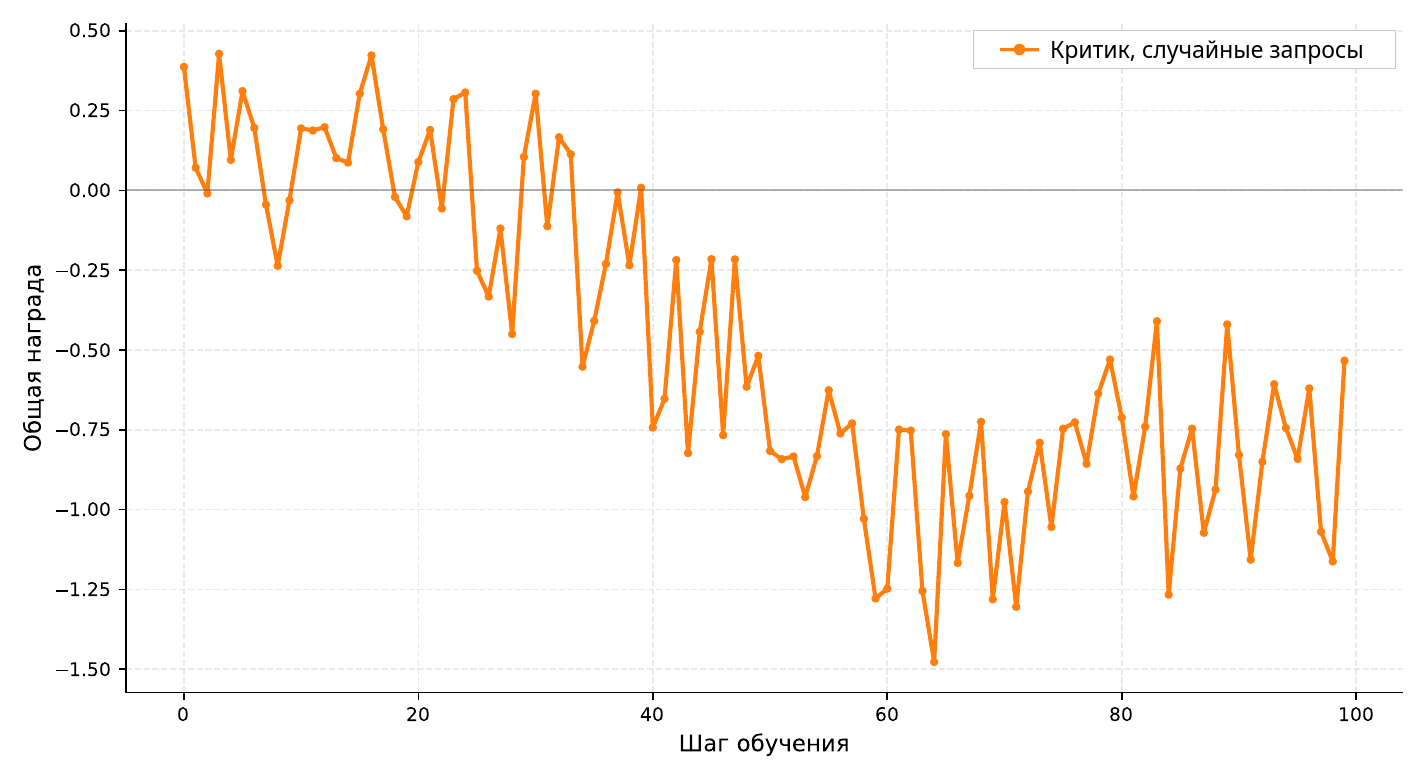
\includegraphics[width=0.82\linewidth]{broad_prompt_ru.png}};
\node[fill=white, minimum width=2.35cm, minimum height=0.28cm, inner sep=0pt] at ($(img.south)+(0,0.24cm)$) {};
\node at ($(img.south)+(0,0.24cm)$) {\scriptsize Эпоха};
\end{tikzpicture}

\medskip
\small
Широкое распределение текстовых запросов делает динамику награды менее устойчивой и хуже интерпретируемой.
\end{frame}

\begin{frame}
\frametitle{А/Б-сравнение с базовой моделью}
\centering

\includegraphics[width=0.82\linewidth]{fixed_prompt_ab/reward_ab_own_metric.pdf}

\medskip
\small
Попарный A/B-тест проводится между базовой и дообученной моделью по той награде, по которой выполнялось дообучение.
\end{frame}

\begin{frame}
\frametitle{Внешняя оценка}
\begin{itemize}
    \item MIDI переводились в ABC-нотацию и оценивались внешней языковой моделью.
    \item Сравнивались базовая модель и схема ``правила затем критик''.
\end{itemize}

\medskip
\centering
\small
\begin{tabular}{lccc}
\toprule
\textbf{Модель} & \textbf{Средняя} & \textbf{Медиана} & \textbf{Макс.} \\
\midrule
Базовая модель & 1.90 & 2.00 & 6.00 \\
После правил и критика & 2.80 & 2.00 & 9.00 \\
\bottomrule
\end{tabular}
\end{frame}

\begin{frame}
\frametitle{Анализ ошибок и ограничений}
\begin{itemize}
    \item Плотность нот легко переоптимизировать.
    \item Базовая модель иногда создаёт пустые или преимущественно ударные дорожки.
    \item Сигнал критика шумнее правил и требует стабилизации.
    \item Запросы лучше усложнять постепенно, иначе сигнал становится слишком неоднородным.
\end{itemize}
\end{frame}

\begin{frame}
\frametitle{Выводы}
\begin{itemize}
    \item Реализован полный цикл GRPO-дообучения \textit{Text2midi}.
    \item Награды на основе правил дают интерпретируемый диагностический сигнал.
    \item Сигнал критика полезен, но требует стабилизации.
    \item Главные ограничения: шум награды, запросы и переоптимизация отдельных признаков, слабость базовой модели
\end{itemize}
\end{frame}

\begin{frame}
\frametitle{Appendix}
\framesubtitle{Распределения тональностей и ладов}
\vspace{0.05cm}
\begin{columns}[c,totalwidth=\textwidth]
	\column{0.5\textwidth}
	\begin{center}
		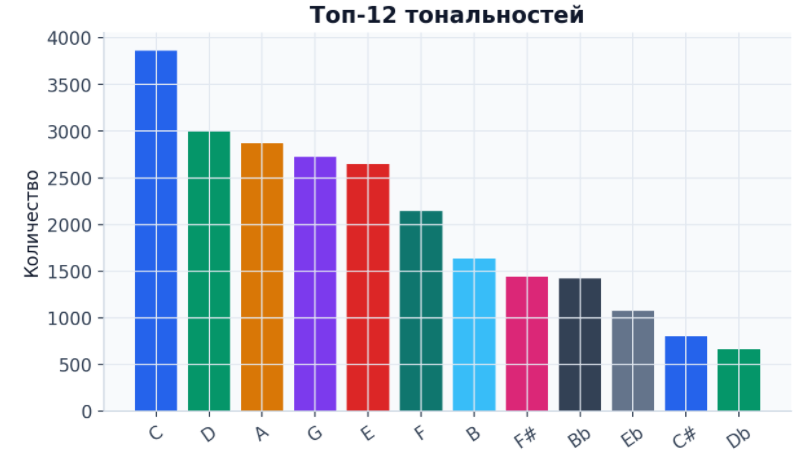
\includegraphics[width=0.96\columnwidth,height=0.62\textheight,keepaspectratio]{key_distribution.png}\\[0.12cm]
		{\fontsize{10}{12}\selectfont \textbf{Распределение тональностей}}
	\end{center}
	\column{0.5\textwidth}
	\begin{center}
		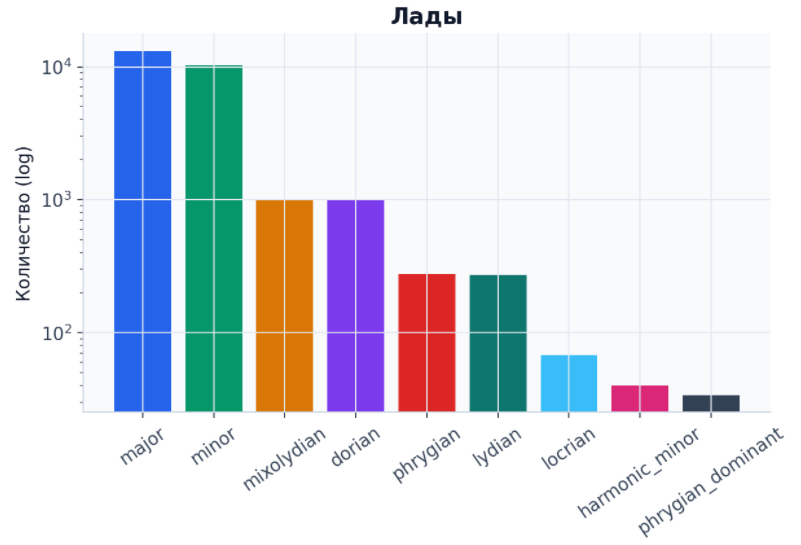
\includegraphics[width=0.96\columnwidth,height=0.62\textheight,keepaspectratio]{mode_distribution.png}\\[0.12cm]
		{\fontsize{10}{12}\selectfont \textbf{Распределение ладов}}
	\end{center}
\end{columns}
\end{frame}

\begin{frame}
\frametitle{Appendix}
\framesubtitle{Распределения ступеней и типов аккордов}
\vspace{0.05cm}
\begin{columns}[c,totalwidth=\textwidth]
	\column{0.5\textwidth}
	\begin{center}
		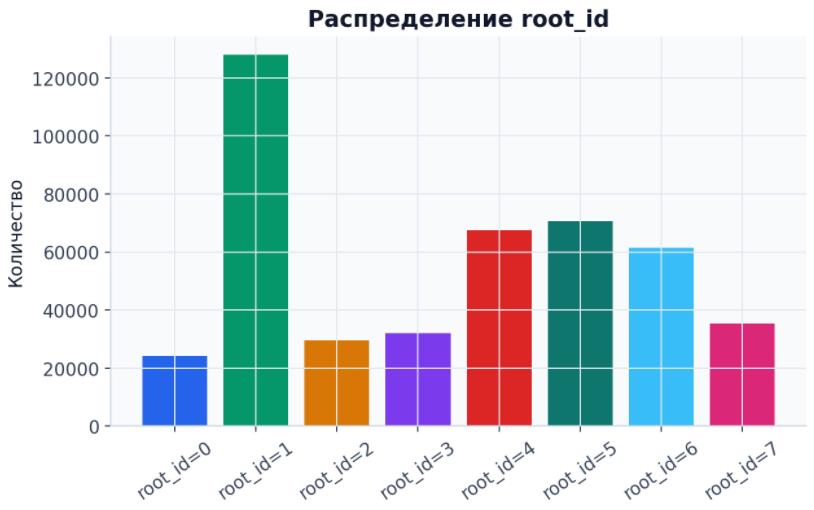
\includegraphics[width=0.96\columnwidth,height=0.62\textheight,keepaspectratio]{chord_degree_distribution.png}\\[0.12cm]
		{\fontsize{10}{12}\selectfont \textbf{Распределение ступеней аккордов}}
	\end{center}
	\column{0.5\textwidth}
	\begin{center}
		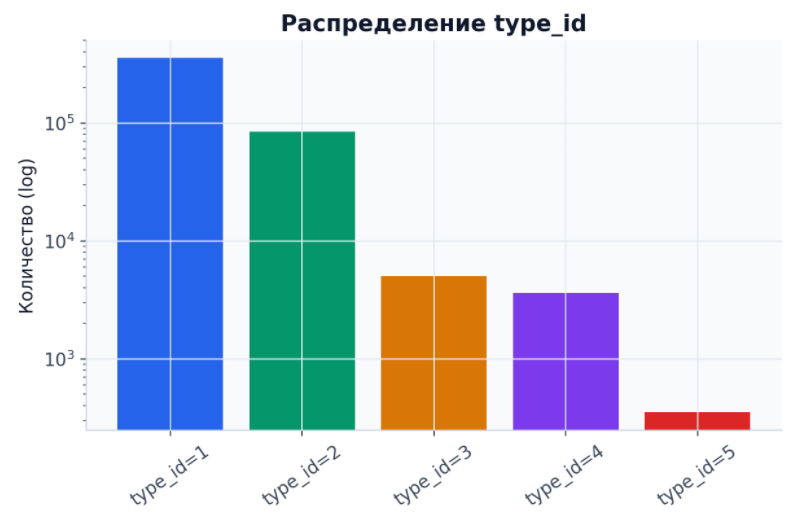
\includegraphics[width=0.96\columnwidth,height=0.62\textheight,keepaspectratio]{chord_type_distribution.png}\\[0.12cm]
		{\fontsize{10}{12}\selectfont \textbf{Распределение типов аккордов}}
	\end{center}
\end{columns}
\end{frame}

\begin{frame}
\frametitle{Appendix}
\framesubtitle{Обучение графового учителя}
\vspace{-0.25cm}
{\fontsize{5.7}{6.5}\selectfont
\setlength{\abovedisplayskip}{1pt}
\setlength{\belowdisplayskip}{1pt}
\begin{columns}[T,totalwidth=\textwidth]
	\column{0.49\textwidth}
	Признаки каждой вершины проецируются в общее скрытое пространство:
	\[
	h_v^{(0)}=\phi_{\tau_v}(x_v),
	\]
	где $\phi_{\tau_v}$ --- \textit{encoder} для типа вершины $\tau_v$, реализованный как \textit{MLP}.

	Для каждого типа ребра $r$ сообщения вычисляются отдельно:
	\[
	m_{u\to v}^{(l,r)}=W_r^{(l)}h_u^{(l)}.
	\]
	Сообщения от соседей агрегируются:
	\[
	m_v^{(l)}=\sum_{r\in R}\operatorname{AGG}_{u\in N_r(v)} m_{u\to v}^{(l,r)}.
	\]
	Состояние вершины обновляется с \textit{residual}-связью, нормализацией и нелинейностью:
	\[
	h_v^{(l+1)}=\operatorname{ReLU}\!\left(\operatorname{LN}\!\left(h_v^{(l)}+m_v^{(l)}\right)\right).
	\]

	После нескольких \textit{GNN}-слоёв модель получает контекстуализированные представления узлов. Затем выполняется \textit{pooling} по типам вершин:
	\[
	g_t=\frac{1}{|V_t|}\sum_{v\in V_t}h_v^{(L)},
	\]
	где $V_t$ --- множество вершин типа $t$.

	\column{0.49\textwidth}
	После объединения векторов разных типов получается общий \textit{embedding} графа:
	\[
	g=\psi\!\left(g_1\Vert g_2\Vert\ldots\Vert g_T\right),
	\]
	где $\Vert$ --- конкатенация, а $\psi$ --- линейная проекция или \textit{MLP}. Итоговая оценка графа:
	\[
	s_\theta(\mathcal{G})=f_{\mathrm{score}}(g).
	\]

	Для обучения используется \textit{contrastive ranking loss}:
	\[
	\mathcal{L}_{\mathrm{rank}}=
	\operatorname{softplus}\!\left(-\left(s_\theta(\mathcal{G})-s_\theta(\widetilde{\mathcal{G}})-m\right)\right),
	\]
	где $m$ --- \textit{margin}. Функция штрафует модель, если \textit{score} искажённого графа слишком близок к \textit{score} исходного или превосходит его.

	Дополнительно может использоваться бинарная классификационная компонента:
	\[
	\mathcal{L}_{\mathrm{bin}}=\frac{1}{2}\left(
	\operatorname{BCE}\!\left(s_\theta(\mathcal{G}),1\right)+
	\operatorname{BCE}\!\left(s_\theta(\widetilde{\mathcal{G}}),0\right)
	\right).
	\]
	Общая функция потерь учителя:
	\[
	\mathcal{L}_{\mathrm{teacher}}=
	\lambda_{\mathrm{rank}}\mathcal{L}_{\mathrm{rank}}+
	\lambda_{\mathrm{bin}}\mathcal{L}_{\mathrm{bin}}+
	\lambda_{\mathrm{local}}\mathcal{L}_{\mathrm{local}}+
	\lambda_{\mathrm{rec}}\mathcal{L}_{\mathrm{rec}}.
	\]
\end{columns}
}
\end{frame}

\begin{frame}
\frametitle{Appendix}
\framesubtitle{Обучение графового ученика}
\vspace{-0.25cm}
{\fontsize{6.1}{7}\selectfont
\setlength{\abovedisplayskip}{1pt}
\setlength{\belowdisplayskip}{1pt}
\begin{columns}[T,totalwidth=\textwidth]
	\column{0.49\textwidth}
	После построения \textit{MIDI}-графа ученик использует компактную гетерогенную \textit{GNN}. Для каждой вершины строится начальное представление:
	\[
	z_v^{(0)}=\phi_{\tau_v}(x_v),
	\]
	после чего несколько графовых слоёв обновляют его через сообщения от соседей:
	\[
	z_v^{(l+1)}=\sigma\!\left(\operatorname{LN}\!\left(
	z_v^{(l)}+\sum_r\operatorname{AGG}_{u\in N_r(v)}W_r^{(l)}z_u^{(l)}
	\right)\right).
	\]
	Далее применяется \textit{pooling} по вершинам и строится \textit{embedding} \textit{MIDI}-графа:
	\[
	z_G=\operatorname{Pool}\!\left(\{z_v^{(L)}\}_{v\in V_M}\right).
	\]
	Итоговая оценка ученика равна:
	\[
	s_\varphi(\mathcal{G}_M)=f_{\mathrm{student}}(z_G).
	\]

	\column{0.49\textwidth}
	Ученик обучается не на ручных метках, а на оценках учителя. Если учитель присваивает музыкальному фрагменту \textit{score} $s_\theta(\mathcal{G})$, то ученик минимизирует ошибку дистилляции:
	\[
	\mathcal{L}_{\mathrm{distill}}=
	\left|s_\varphi(\mathcal{G}_M)-s_\theta(\mathcal{G})\right|,
	\]
	или её сглаженный вариант:
	\[
	\mathcal{L}_{\mathrm{distill}}=
	\operatorname{SmoothL1}\!\left(s_\varphi(\mathcal{G}_M),s_\theta(\mathcal{G})\right).
	\]
	Для пар \textit{clean/corrupted} дополнительно используется \textit{ranking loss}:
	\[
	\mathcal{L}_{\mathrm{student\text{-}rank}}=
	\operatorname{softplus}\!\left(-\left(s_\varphi(\mathcal{G}_M)-s_\varphi(\widetilde{\mathcal{G}}_M)\right)\right).
	\]
\end{columns}
}
\end{frame}

\begin{frame}
\frametitle{Appendix}
\framesubtitle{Положительная часть аккордового score}
\hypertarget{positive-score}{}
\vspace{-0.15cm}
{\fontsize{9.5}{11.5}\selectfont
\textbf{Компоненты положительной части аккордового \textit{score}}\\[0.08cm]
\setlength{\tabcolsep}{4pt}
\renewcommand{\arraystretch}{1.18}
\begin{tabular}{@{}p{0.34\textwidth}p{0.58\textwidth}@{}}
\toprule
\textit{Компонента} & \textit{Интерпретация} \\
\midrule
$\operatorname{mode\_match}(c)$ & Совпадение лада \\
$\operatorname{bass\_match}(c)$ & Совпадение басовой ноты \\
$|P_w \cap B(c)|$ & Количество совпадающих нот \\
$\operatorname{explained\_extras}(c, P_w)$ & Надстройки \\
\bottomrule
\end{tabular}
}
\end{frame}

\begin{frame}
\frametitle{Appendix}
\framesubtitle{Штрафная часть аккордового score}
\hypertarget{negative-score}{}
\vspace{-0.1cm}
{\fontsize{9.5}{11.5}\selectfont
\textbf{Компоненты штрафной части аккордового \textit{score}}\\[0.08cm]
\setlength{\tabcolsep}{4pt}
\renewcommand{\arraystretch}{1.22}
\begin{tabular}{@{}p{0.38\textwidth}p{0.56\textwidth}@{}}
\toprule
\textit{Компонента} & \textit{Интерпретация} \\
\midrule
$\operatorname{Unexplained}(c, P_w)$ & Ноты которые не объясняются кандидатом \\
$\operatorname{MissingCore}(c, P_w)$ & Ноты кандидата которых нет в MIDI \\
$\operatorname{borrowed\_mode\_penalty}(c)$ & Штраф за заимствованный лад \\
$\operatorname{mode\_distance}(c)$ & Штраф за расстояние до заимствованного лада \\
$\operatorname{body\_size\_penalty}(c)$ & Штраф за размер аккорда \\
$\operatorname{complexity\_penalty}(c)$ & Штрафы за добавленные ступени, задержания, альтерации и пропущенные обязательные тона. \\
\bottomrule
\end{tabular}
}
\end{frame}

\begin{frame}
\frametitle{Appendix}
\framesubtitle{Пример применения аккордового оценщика}
\vspace{-0.25cm}
{\fontsize{8.5}{10}\selectfont
Пусть в момент времени $t$ наблюдаются \textit{MIDI}-ноты
$C - E - G - B\flat$, тогда $P_t=\{C,E,G,B\flat\}$.
\vspace{0.08cm}
\setlength{\tabcolsep}{2.5pt}
\renewcommand{\arraystretch}{1.16}
\resizebox{\textwidth}{!}{%
\begin{tabular}{@{}p{0.17\textwidth}p{0.29\textwidth}p{0.31\textwidth}p{0.19\textwidth}@{}}
\toprule
\textit{Кандидат} & \textit{Тело аккорда} & \textit{Совпадения и штрафы} & \textit{Итог} \\
\midrule
\textbf{$C7$} &
$B(C7)=\{C,E,G,B\flat\}$ &
$P_t\cap B(C7)=\{C,E,G,B\flat\}$;\newline
$\operatorname{MissingCore}=\varnothing$;\newline
$\operatorname{Unexplained}=\varnothing$ &
Высокий \textit{score}: полный доминантсептаккорд. \\
\midrule
\textbf{$C$ major} &
$B(C)=\{C,E,G\}$ &
Трезвучие объясняется, но $B\flat$ остаётся необъяснённым:\newline
$\operatorname{Unexplained}=\{B\flat\}$ &
\textit{Score} ниже, если $B\flat$ не считается допустимой добавленной или альтерированной ступенью. \\
\midrule
\textbf{$Am7\flat5/C$} &
$B(Am7\flat5)=\{A,C,E\flat,G\}$ &
Есть $C$ и $G$, но отсутствуют $A$ и $E\flat$; вместо $E\flat$ наблюдается $E$:\newline
$\operatorname{MissingCore}=\{A,E\flat\}$ &
Совпадение баса $C$ не компенсирует штрафы: \textit{score} ниже, чем у $C7$. \\
\bottomrule
\end{tabular}%
}
}
\end{frame}

\end{document}
